%!TEX root = ../slides.tex
%\begin{frame}
%  \vfill
%  \centering
%  %\begin{beamercolorbox}[sep=8pt,center,shadow=true,rounded=true]{block}
%  \begin{sticky}
%    \usebeamerfont{title}
%    {\normalfont\Large MultiParty Session Types} \par%
%  \end{sticky}
%  %\end{beamercolorbox}
%  \vfill
%\end{frame}
%
\begin{frame}
  \vfill
  \centering
  %\begin{beamercolorbox}[sep=8pt,center,shadow=true,rounded=true]{block}
  \begin{sticky}
    \usebeamerfont{title}
    {\normalfont \textbf{Background and Motivation}}

    {\normalfont\Large A Crash Course on Classic Multiparty Session Types}
    \par%
  \end{sticky}
  %\end{beamercolorbox}
  \vfill
\end{frame}

\begin{frame}[fragile]{What is wrong with this code?}
  \scriptsize
  \begin{lstlisting}[language=Golang,
  belowskip=-0.6\baselineskip, aboveskip=-0.1\baselineskip]
func Worker(n int, resp chan int, err chan error) { ... }
func Master(reqCh chan int, respCh chan []int, cErrCh chan error) {
  for {
    ubound := <-reqCh
    workerChs := make([]chan int, ubound)
    errCh := make(chan error)
    for i := 0; i < ubound; i++ {
      workerChs[i] = make(chan int)
      go Worker(i+1, workerChs[i], errCh)
    }
    var res []int
    for i := 0; i < ubound; i++ {
      select {
      case sqI := <-workerChs[i]:
        res = append(res, sqI)
      case err := <-errCh:
        cErrCh <- err
        return
      }}
    respCh <- res}}
\end{lstlisting}
  \Put(40,290){%
    \begin{onlyenv}<2>
    \begin{minipage}{.86\columnwidth}
    \begin{infobox}
      \Large
      \textbf{DEADLOCK!}\vspace{.2cm}\\
      \textbf{ORPHAN MESSAGES!}\vspace{.2cm}\\
      \textbf{NO RESOURCE CLEANUP!}\vspace{.2cm}\\
      \textbf{...}
    \end{infobox}
    \end{minipage}
    \end{onlyenv}
    \begin{onlyenv}<3>
    \begin{minipage}{.86\columnwidth}
    \begin{greenbox}
      \Large
       \lstinline{Master} needs to guarantee that all \lstinline{Worker}s are
       notified when there is an error.
    \end{greenbox}
    \end{minipage}
    \end{onlyenv}
  }
\end{frame}

\begin{frame}[fragile]{Key Idea}
  Multiparty Session Types prevent you from writing the code in the previous
  slide by enforcing \underline{syntactically} that process implementations
  follow a given specification.

  \vspace{1cm}
  \textbf{In a nutshell:}
  \begin{enumerate}
    \item \underline{Global types:} protocol specifications among a fixed number of different \emph{roles}.
    \item \underline{Role:} sets of interactions that processes can do in a protocol.
    \item \underline{Local types:} protocol specifications \emph{from the point of view of a single role}.
    \item \underline{Projection:} a \emph{partial function} that extracts
      \emph{local type} given a \emph{global types} and a \emph{role}.
    \item[]
    \item \underline{Well-formedness:} guarantees \textbf{deadlock-freedom},
      usually defined in terms of \emph{projectibility}.
  \end{enumerate}
\end{frame}

\begin{frame}
  \vskip.1cm
  \begin{center}
  \only<1>{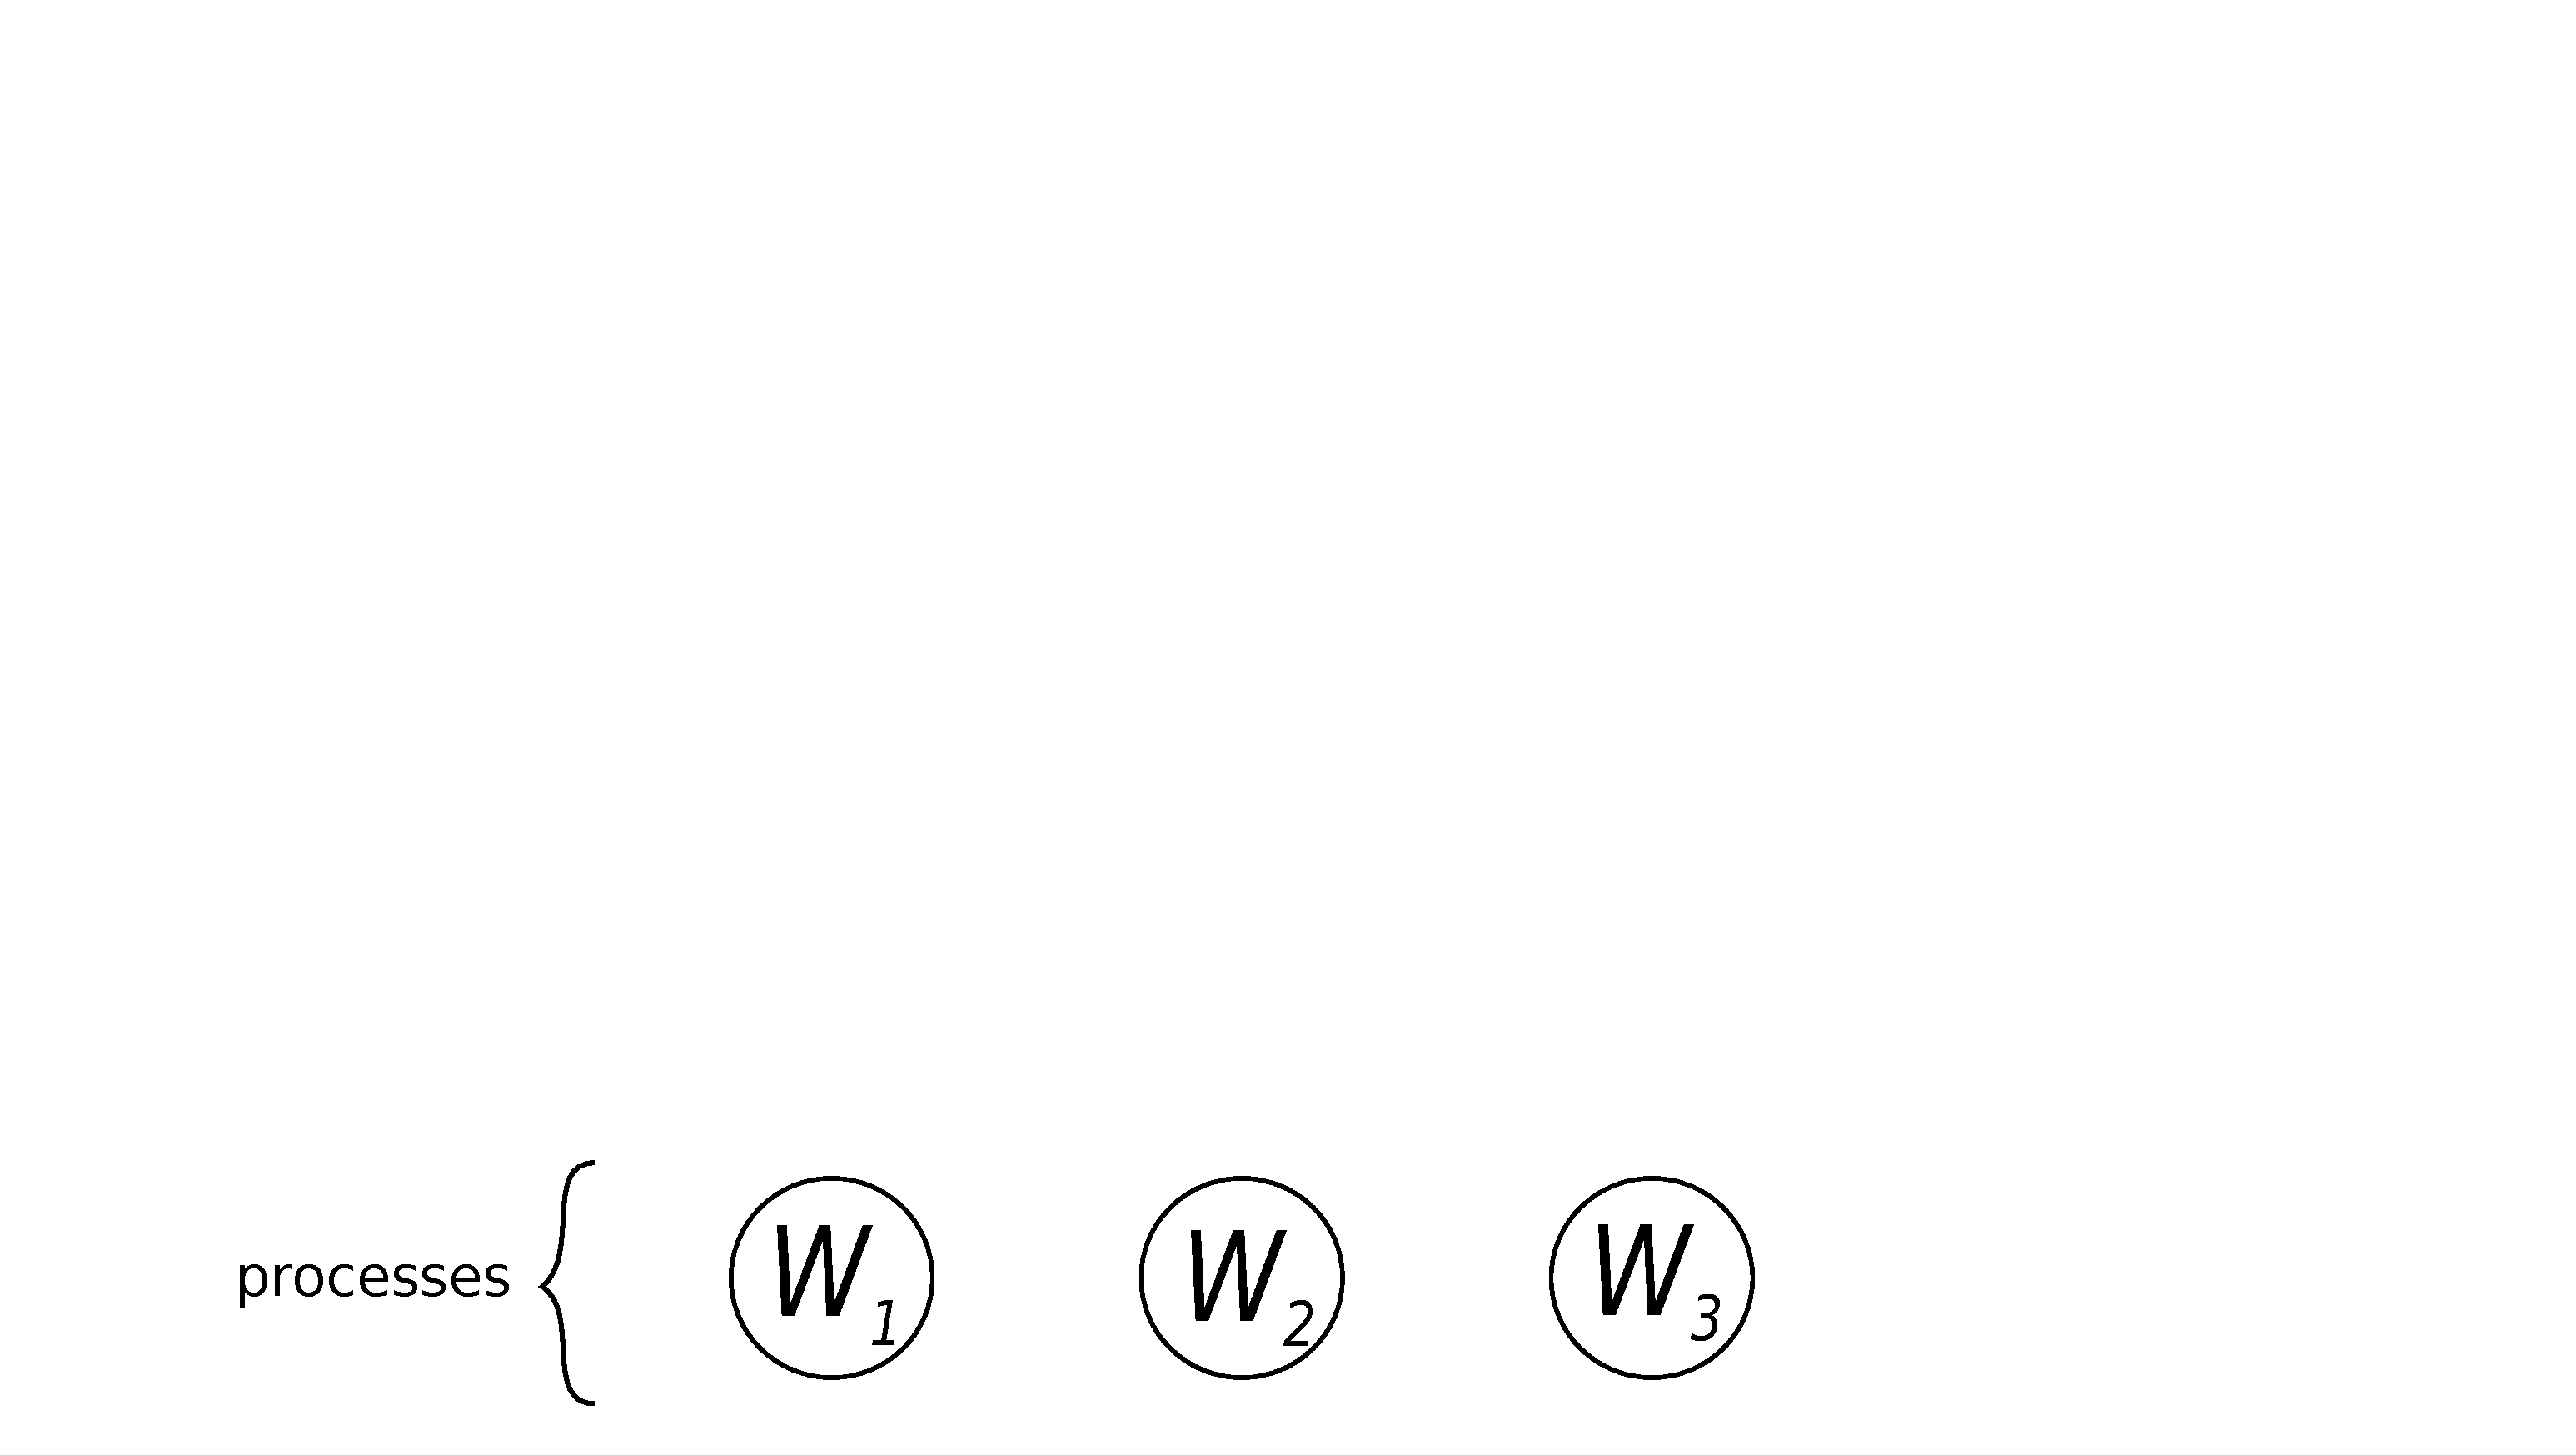
\includegraphics[width=.8\textwidth]{figures/MPST1.pdf}}%
  \only<2>{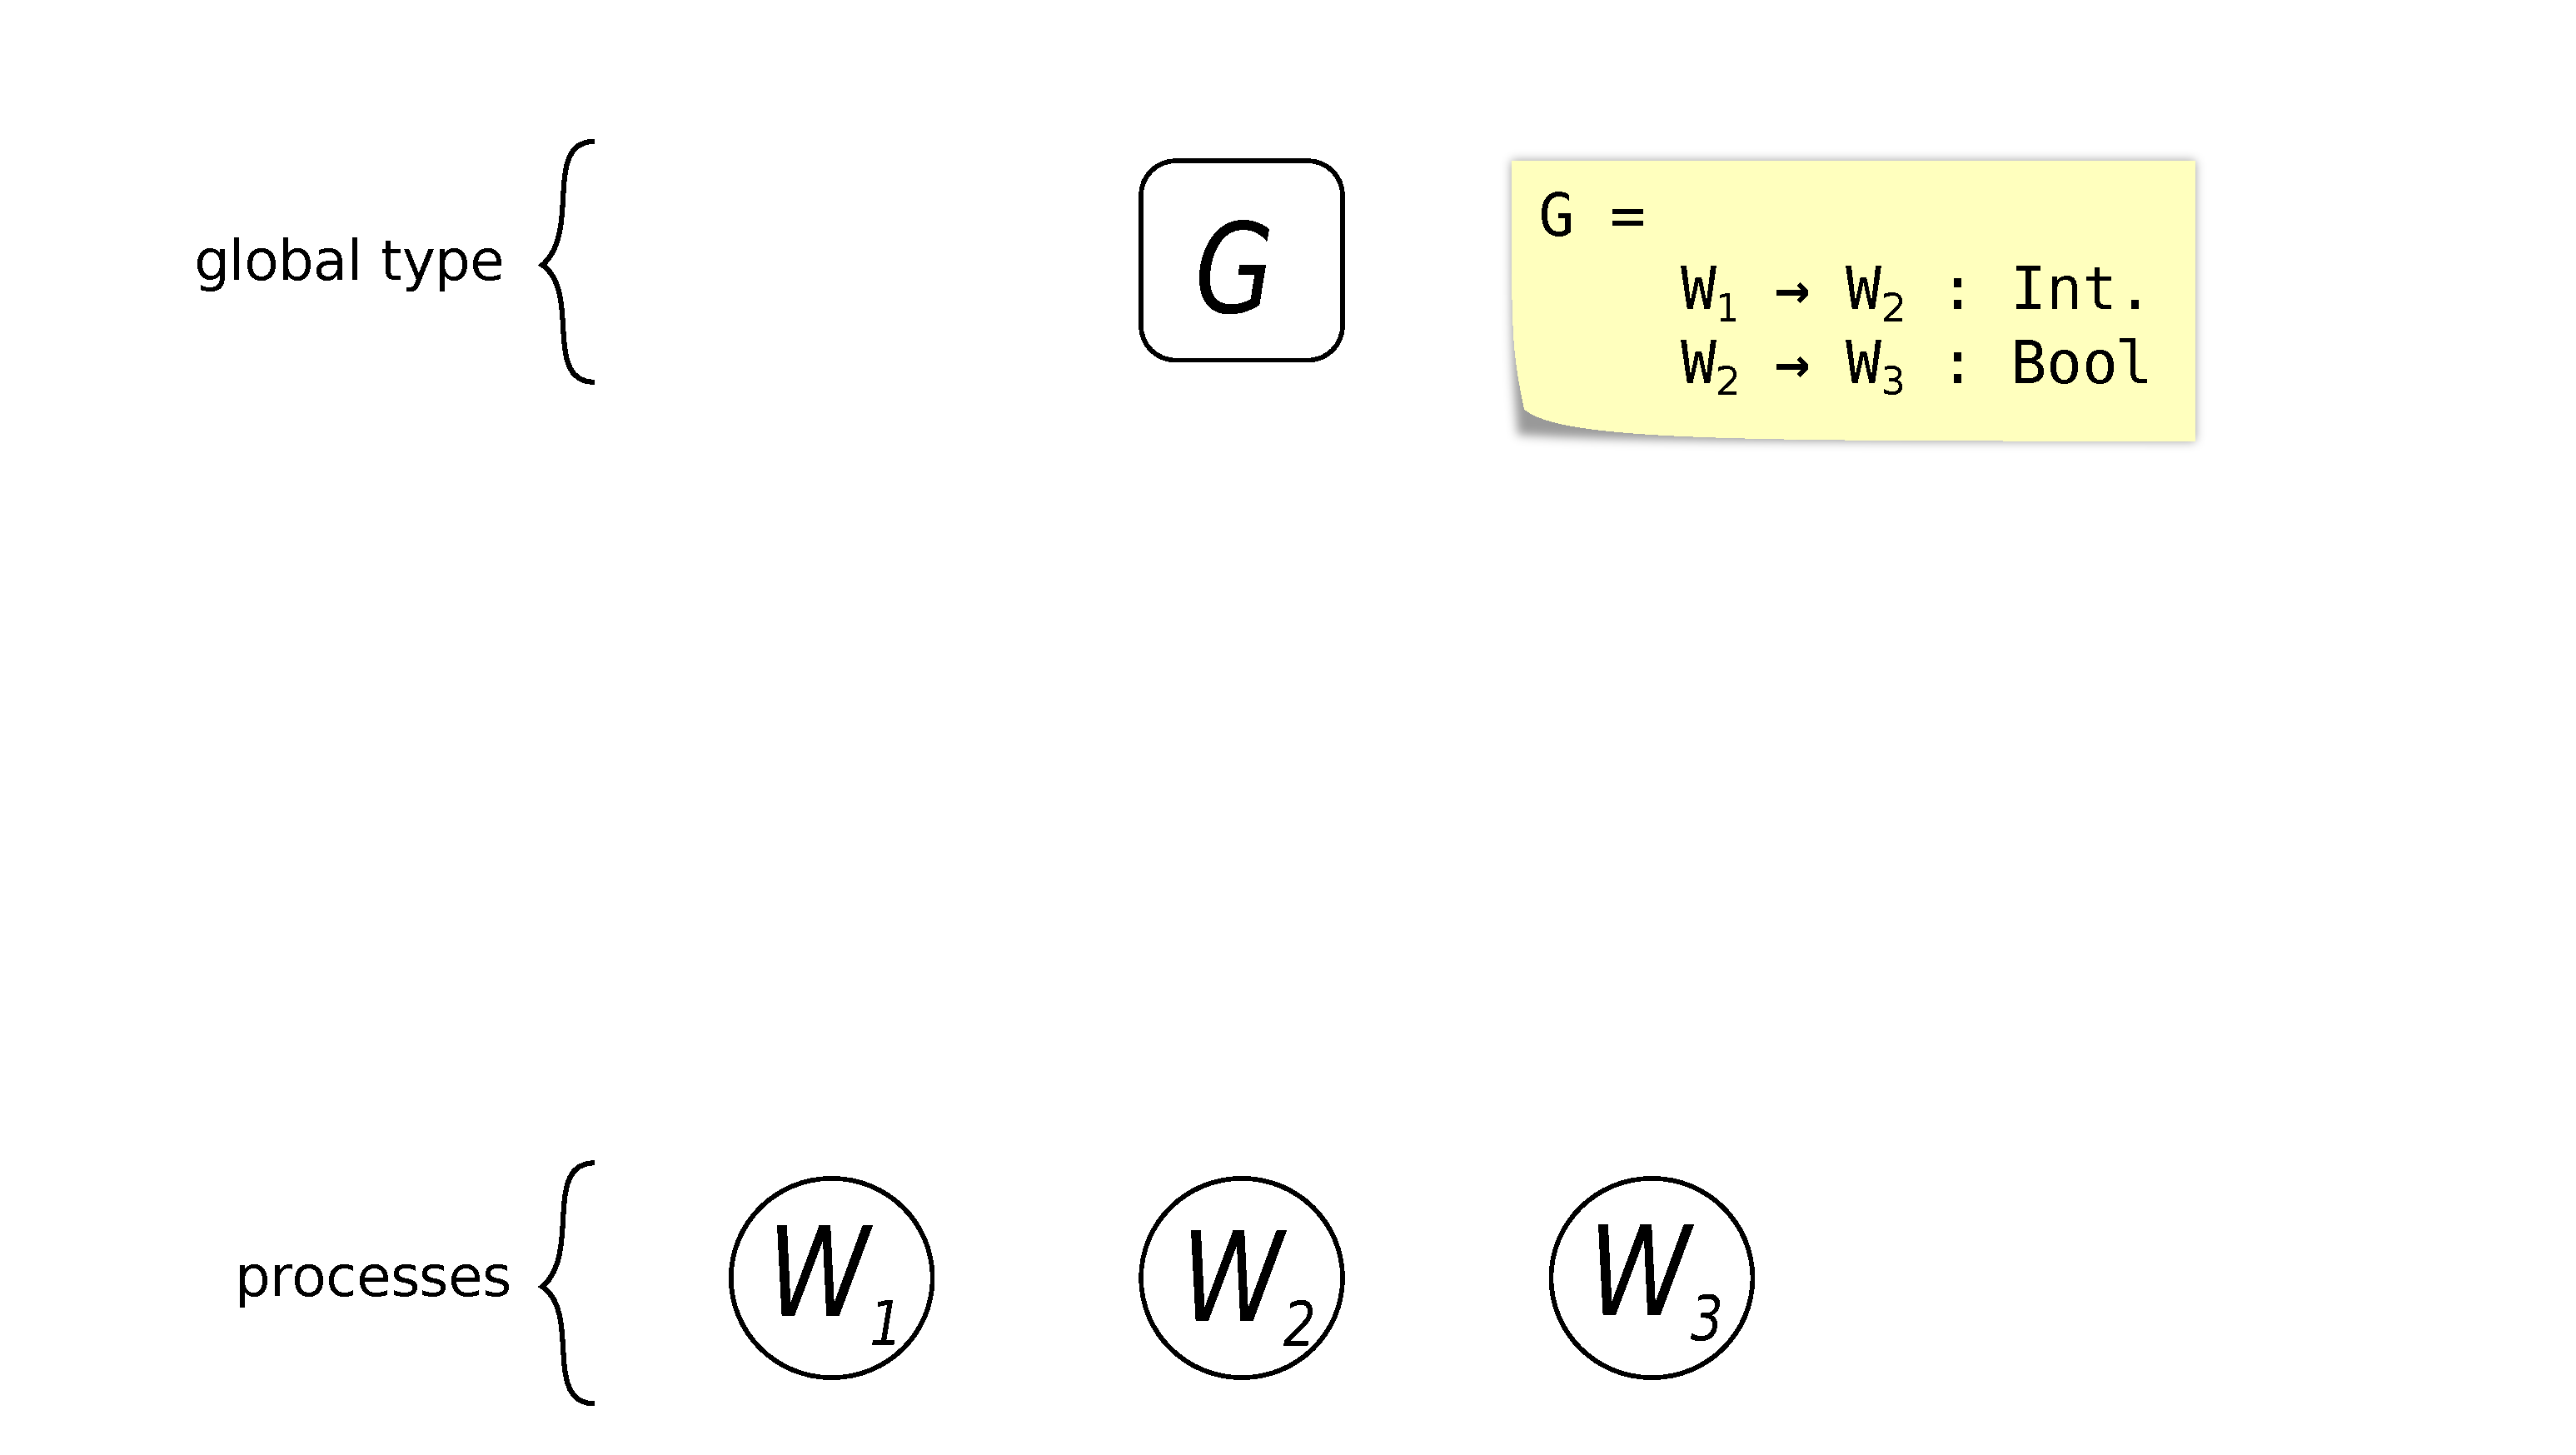
\includegraphics[width=.8\textwidth]{figures/MPST2.pdf}}%
  \only<3>{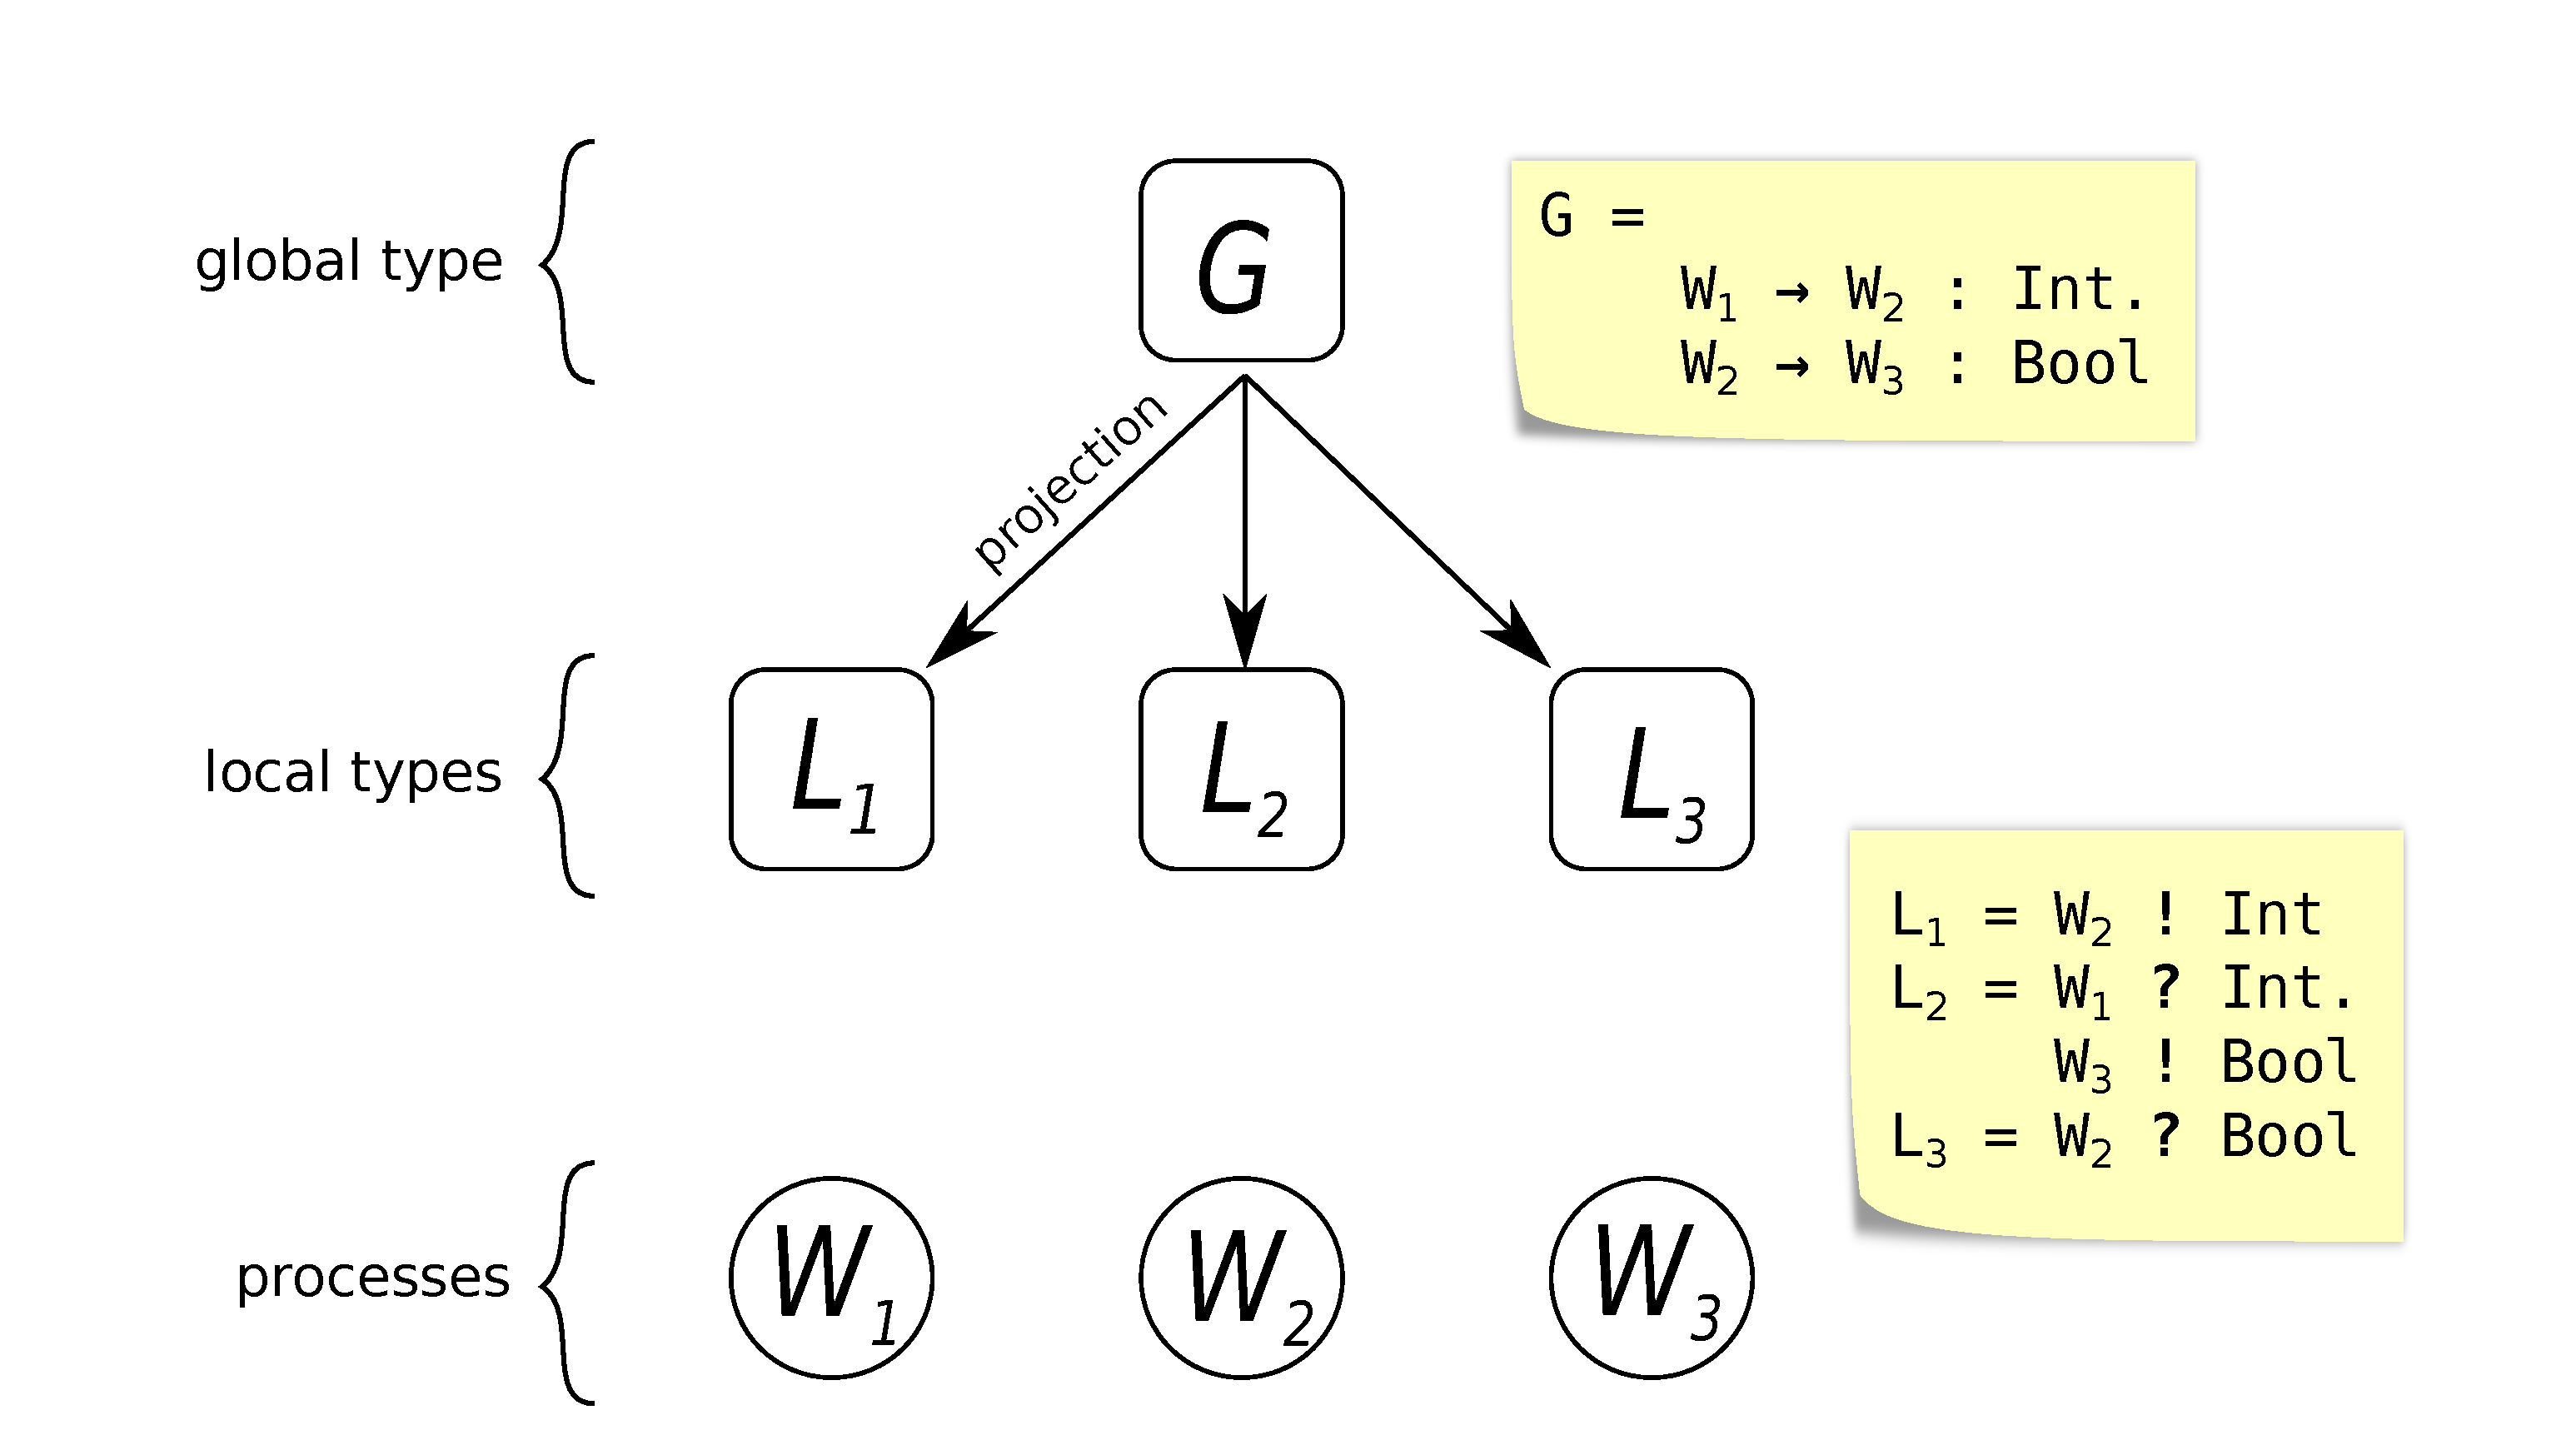
\includegraphics[width=.8\textwidth]{figures/MPST3.pdf}}%
  \only<4>{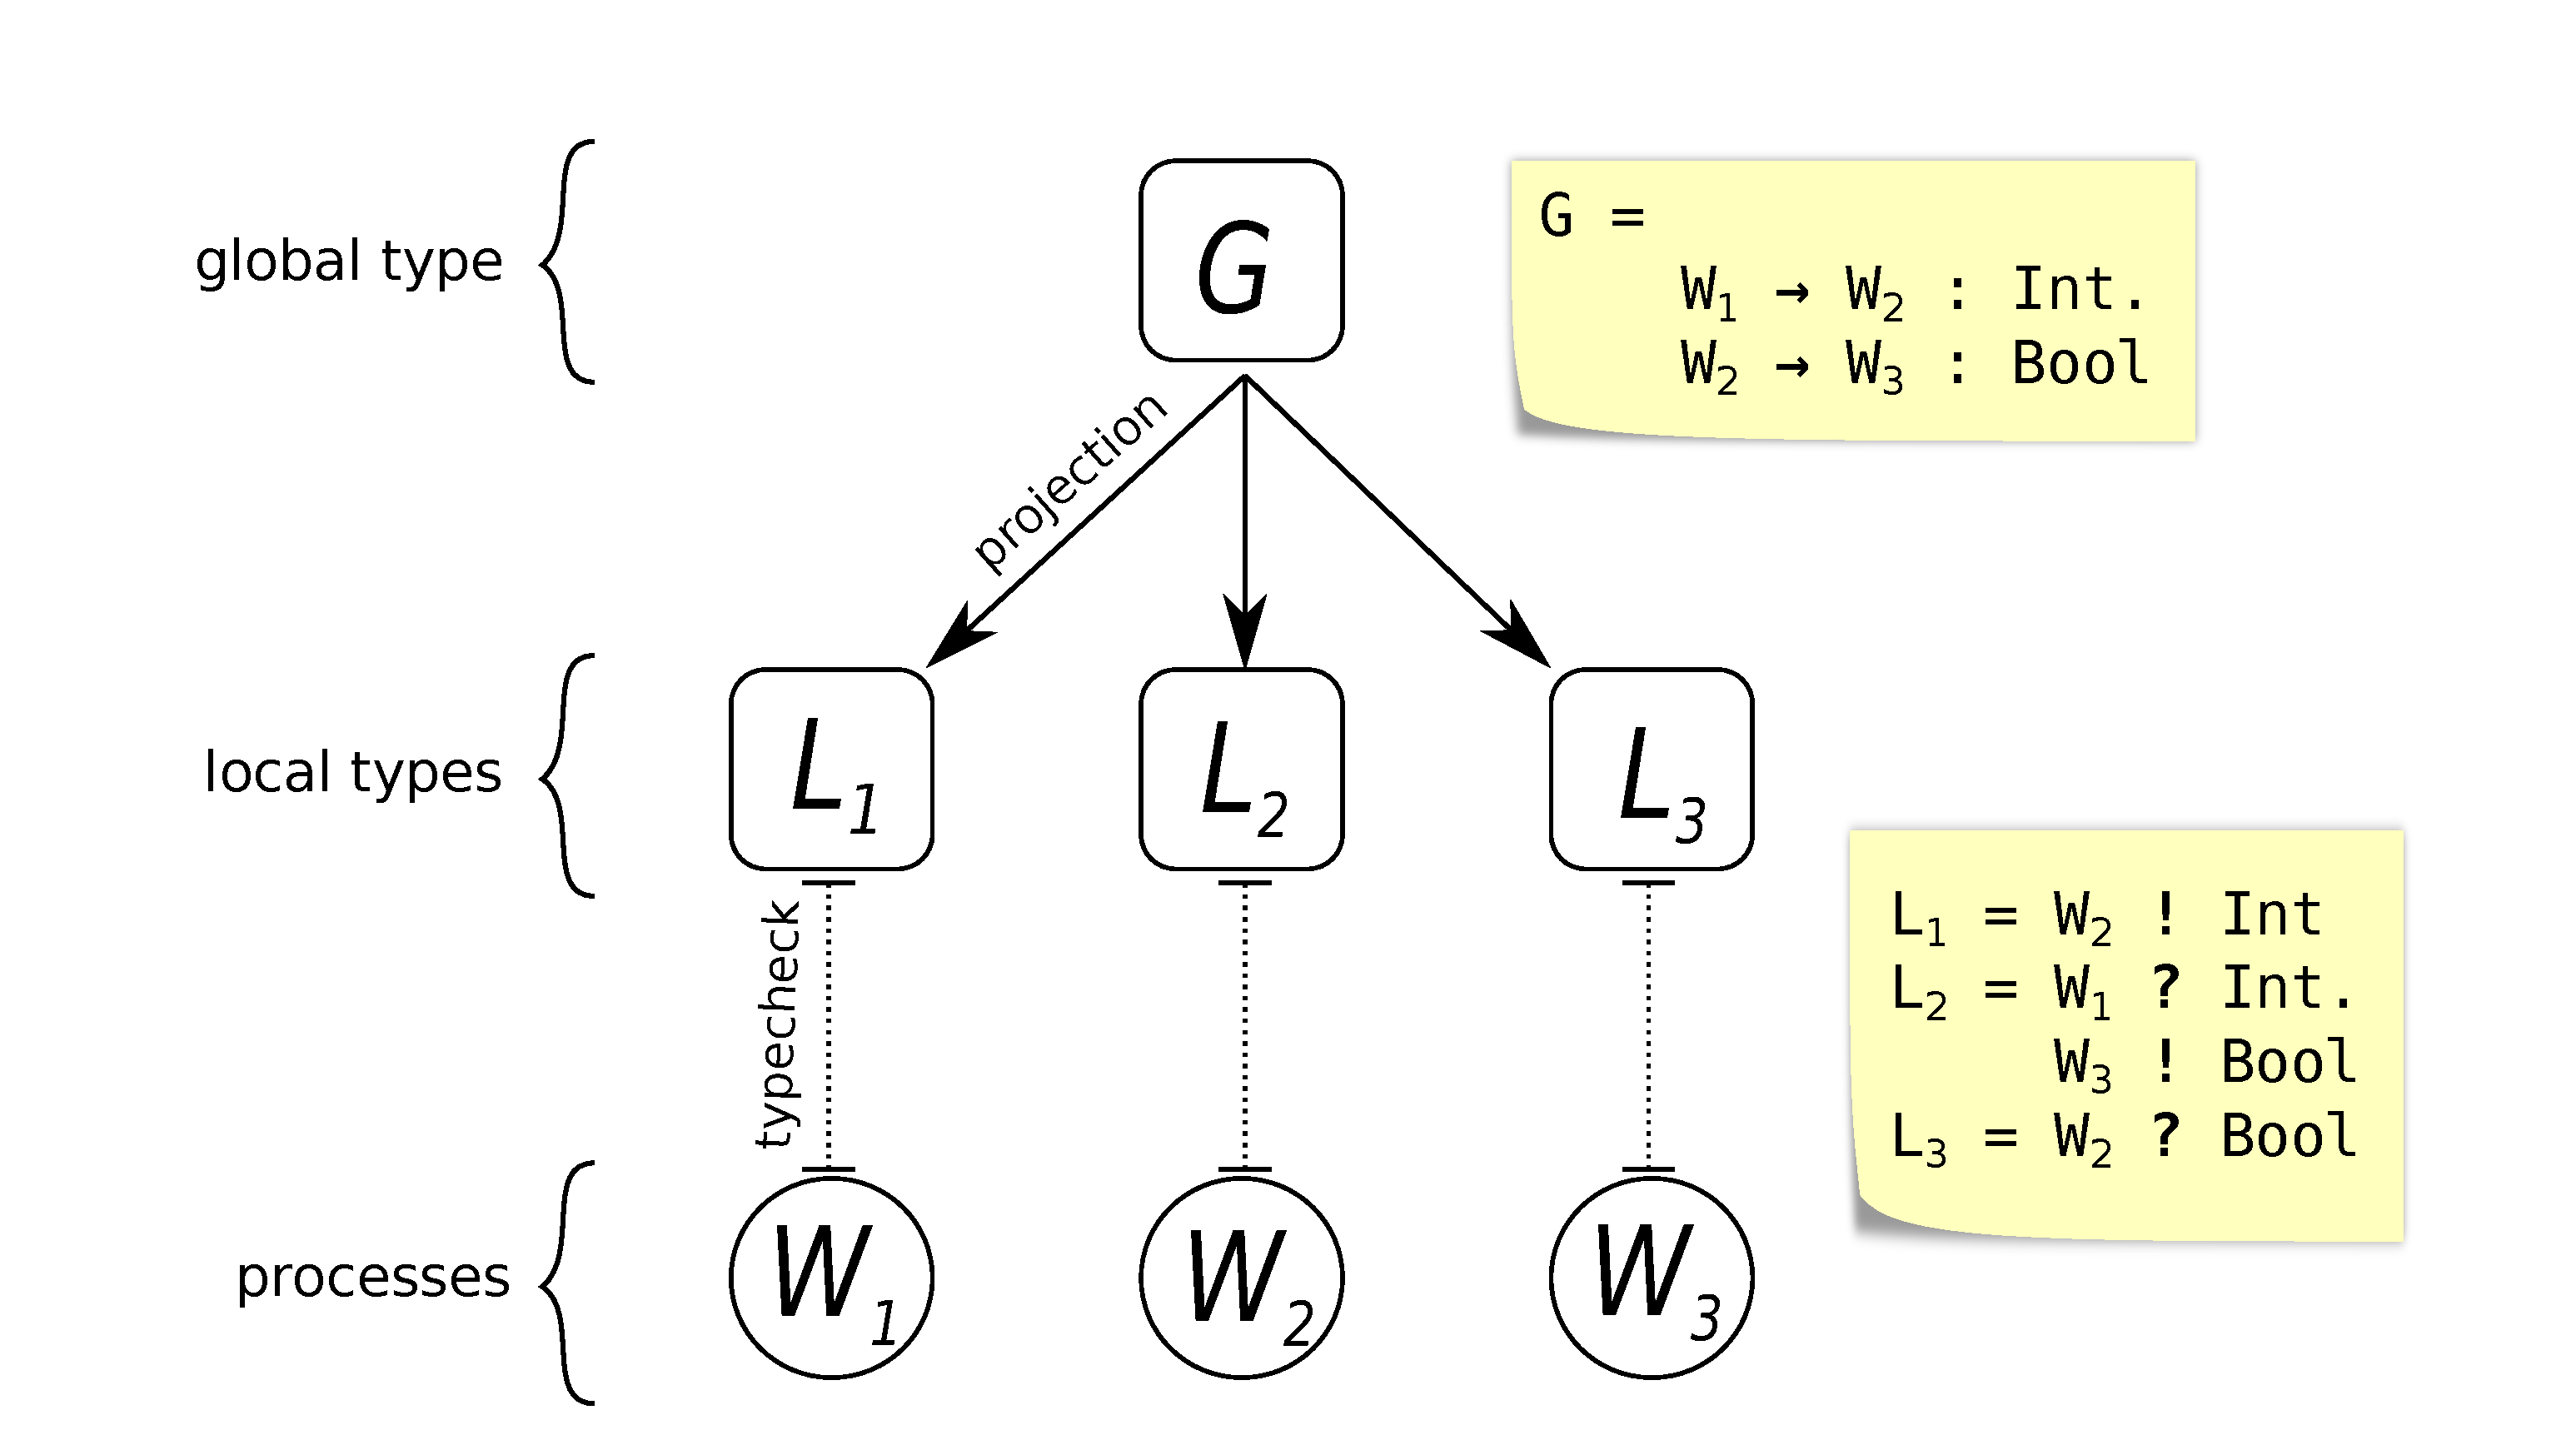
\includegraphics[width=.8\textwidth]{figures/MPST4.pdf}}%
  \only<5>{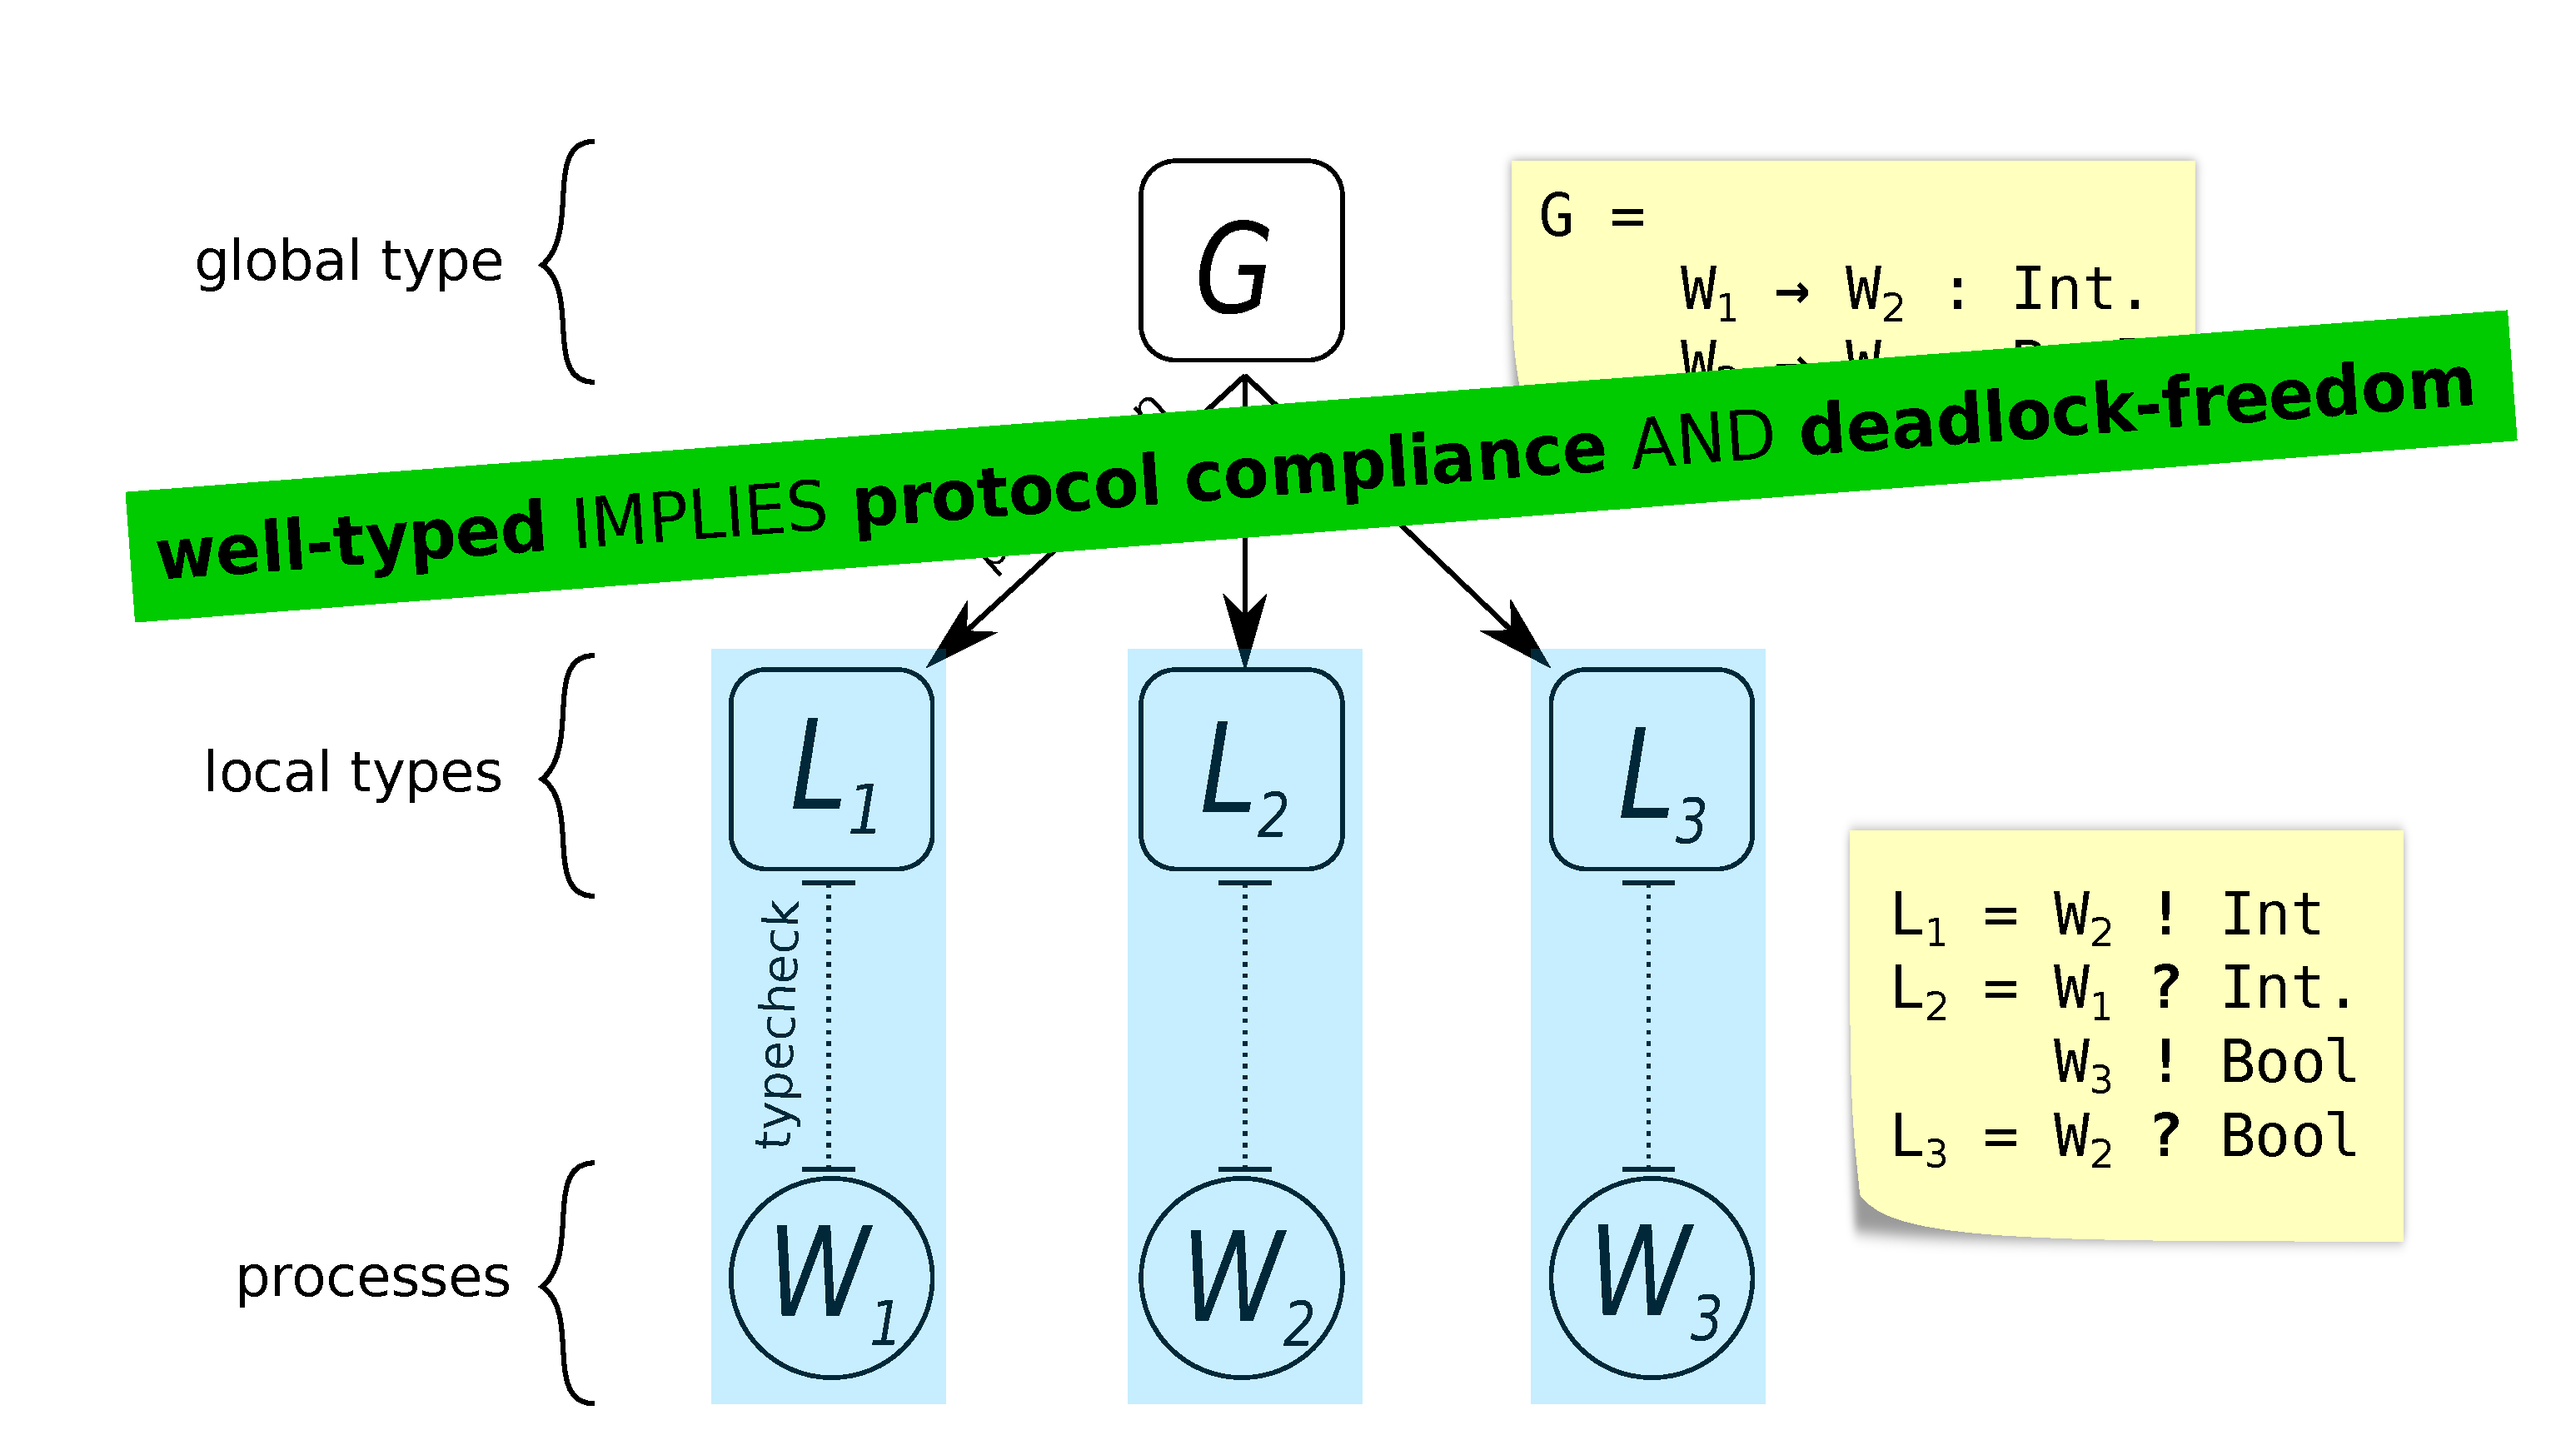
\includegraphics[width=.8\textwidth]{figures/MPST5.pdf}}
  \end{center}
\end{frame}

\begin{frame}{Global and Local Types}
\begin{displaymath}
  \begin{array}{lrcll}
    \text{Roles} &  &  & \Rp, \Rq, \ldots &  \\\\
    \text{Sorts} & \expt{S} & \mathrel{:=} & \sbool \mid \snat \mid \cdots & \text{Basic data types.} \\\\
    \text{Global Types} & \globalt{G} & \mathrel{:=}
    & \gmsg \Rp \Rq {{\gmsgbr {\lbl_i} {S_i} {G_i}}_{i\in I}} & \text{Message communication.} \\
    & & \mid & \grecur X G & \text{Recursion.} \\
    & & \mid & \pvar X & \text{Recursion variable.} \\
    & & \mid & \gfinish & \text{End of protocol.} \\\\
    \text{Local Types} & \localt{L} & \mathrel{:=}
    & \lsend \Rp {{\lmsgbr {\lbl_i} {S_i} {L_i}}_{i\in I}} & \text{Send message.} \\
    & & \mid & \lrecv \Rq {{\lmsgbr {\lbl_i} {S_i} {L_i}}_{i\in I}} & \text{Receive message.} \\
    & & \mid & \lrecur X G & \text{Recursion.} \\
    & & \mid & \pvar X & \text{Recursion variable.} \\
    & & \mid & \lfinish & \text{End of protocol.} \\
  \end{array}
\end{displaymath}

\end{frame}

\begin{frame}{Projection}

\begin{displaymath}
  \begin{array}{c}
\gproj{\gmsg \Rp \Rq {{\gmsgbr {\lbl_i} {S_i} {G_i}}_{i\in I}}}{\Rr} =
\left\{%
\begin{array}{l l}
\lsend \Rq {{\lmsgbr {\lbl_i} {S_i} {\gproj{G_i}{\Rr}}}_{i\in I}} & (\Rr = \Rp \wedge \phantom{\Rr = \Rq} \wedge \Rp \neq \Rq) \\
\lrecv \Rp {{\lmsgbr {\lbl_i} {S_i} {\gproj{G_i}{\Rr}}}_{i\in I}} & (\phantom{\Rr = \Rp} \wedge \Rr = \Rq \wedge \Rp \neq \Rq) \\
\lmerge_{i \in I}(\gproj{G_i}{\Rr}) & (\Rr \neq \Rp \wedge \Rr \neq \Rq \wedge \Rp \neq \Rq) \\
\end{array}
\right.
\\[1cm]
\gproj{\grecur X G}{\Rr} =
\left\{%
\begin{array}{l l}
  \lrecur X {\gproj{G}{\Rr}} & (\Rr \in G) \\
  \lfinish & (\Rr \not\in G)
\end{array}
\right.
\hspace{1cm}
\gproj{\pvar X}{\Rr} = \pvar X
\hspace{1cm}
\gproj{\gfinish}{\Rr} = \lfinish
  \end{array}
\end{displaymath}

\noindent\makebox[\linewidth]{\rule{\columnwidth}{0.4pt}}

\uncover<2->{%
\begin{displaymath}
  \begin{array}{c}
    \begin{array}{l}
\lrecv \Rp {{\lmsgbr {\lbl_i} {S_i} {L_i}}_{i\in I}}
\mathbin{\lmerge}
\lrecv \Rp {{\lmsgbr {\lbl_j} {S_j} {L'_j}}_{j\in J}}
\\\quad
= \lrecv \Rp {{\lmsgbr {\lbl_i} {S_i} {L_i}}_{i\in I\setminus J}
  \cup {\lmsgbr {\lbl_j} {S_j} {L'_j}}_{j\in J\setminus I}
\cup {\lmsgbr {\lbl_i} {S_i} {L_i \mathbin{\lmerge} L'_i}}_{i\in I \cap J}}
\\[.5cm]
\lsend \Rp {{\lmsgbr {\lbl_i} {S_i} {L_i}}_{i\in I}}
\mathbin{\lmerge}
\lsend \Rp {{\lmsgbr {\lbl_i} {S_i} {L'_i}}_{i\in I}}
=
\lsend \Rp {{\lmsgbr {\lbl_i} {S_i} {L_i \lmerge L'_i}}_{i\in I}}
\\[.5cm]
\lrecur X L \mathbin{\lmerge} \lrecur X L' = \lrecur X (L \mathbin{\lmerge} L')
\hspace{1cm}
L \mathbin{\lmerge} L = L
\end{array}
  \end{array}
\end{displaymath}
}
  \Put(40,290){%
    \begin{onlyenv}<3>
    \begin{minipage}{.86\columnwidth}
    \begin{infobox}
      \Large
      \textbf{It gets complicated very quickly!}
    \end{infobox}
    \end{minipage}
    \end{onlyenv}
  }
\end{frame}

\begin{frame}{What is the point of $\lmerge$?}
  Example:

  \begin{displaymath}
    \grecur X {
\gmsg \Rp \Rq {\left\{%
  \begin{array}{l@{}l}
   \dlbl{\mathsf{REQ}}(\snat) &. \gmsg \Rq \Rr {\dlbl{\mathsf{REQ}}(\sbool). \pvar{X}} \\
   \dlbl{\mathsf{END}}() &. \gmsg \Rq \Rr {\dlbl{\mathsf{END}}(). \pfinish}
  \end{array}
   \right\}}}
  \end{displaymath}

  \vspace{1cm}
  \uncover<2->{%
    Projecting $\Rr$
  \begin{displaymath}
    \begin{array}{l}
    \lrecur X {
      (\lrecv \Rq {\dlbl{\mathsf{REQ}}(\sbool). \pvar{X}})
        \mathbin{\lmerge}
      (\lrecv \Rq {\dlbl{\mathsf{END}}(). \lfinish})
   }
    \\[.3cm] \qquad =
    \uncover<3>{%
    \lrecur X {
\lrecv \Rq {\left\{%
  \begin{array}{l@{}l}
   \dlbl{\mathsf{REQ}}(\sbool) &. \pvar{X} \\
   \dlbl{\mathsf{END}}() &. \pfinish
  \end{array}
   \right\}}}
    \end{array}
  \end{displaymath}
  }}

\end{frame}


\begin{frame}{Processes and Typing}

\begin{displaymath}
  \begin{array}{lrcll}
    \text{Process} & \proc{P} & \mathrel{:=} & \psend p \lbl e P & \text{Send a message.} \\
    & & \mid & \precv i I {\precbr p {\lbl_i} {x_i} {P_i}} & \text{Receive a message.} \\
    & & \mid & \pif e P {P'} & \text{Conditional process.} \\
    & & \mid & \precur X P & \text{Recursive process.} \\
    & & \mid & \pvar X & \text{Recursion variable.} \\
    & & \mid & \pfinish & \text{Inactive process.} \\
  \end{array}
\end{displaymath}

\end{frame}

\begin{frame}{Process Typing (simplified)}
  Once we have local types, process typing is simple:
  \vspace{.4cm}

\begin{displaymath}
  \begin{array}{c}
  \infer[T-SEND]
  { \loft \Gamma P {L_i} \and \toft \Gamma e S_i \and i \in I}
  {\loft \Gamma {\psend \Rq {\lbl_i} e P} (\lsend \Rp {{\lmsgbr {\lbl_i} {S_i} {L_i}}_{i\in I}})}
  \hspace{1cm}
  \infer[T-RECV]
  { \loft {\Gamma , {\pvar{x_i}} : {\expt{S_i}}} {P_i} {L_i} \and \forall i \in I}
  {\loft \Gamma {\precv i I {\precbr p {\lbl_i} {x_i} {P_i}}} (\lrecv \Rp {{\lmsgbr {\lbl_i} {S_i} {L_i}}_{i\in I}})}
  \end{array}
\end{displaymath}

\end{frame}

\begin{frame}{Problems with Classic Formulation}
  \begin{enumerate}
    \item \textbf{Too syntactic:}
      \begin{itemize}
        \item Processes and local types must align
        \item Too restrictive, rules out correct processes
        \item \ldots
      \end{itemize}
    \item \textbf{Unnecessarily complex:}
      \begin{itemize}
        \item Hard to implement/mechanise, e.g.:
          \begin{itemize}
            \item Use of runtime coinductive global types: Our PLDI 2021 paper
            \item Complex graph-based representation of MPST: Jacobs et al. (2022)
            \item Graph-based reasoning and decision procedure for the equality
              of recursive types: Tirore et al. (2023)
          \end{itemize}
        \item Hard to extend
      \end{itemize}
  \end{enumerate}
\end{frame}

\begin{frame}{A Few Attempts at Simplifying the Theory}

    \begin{minipage}{.86\columnwidth}
    \begin{sticky}
  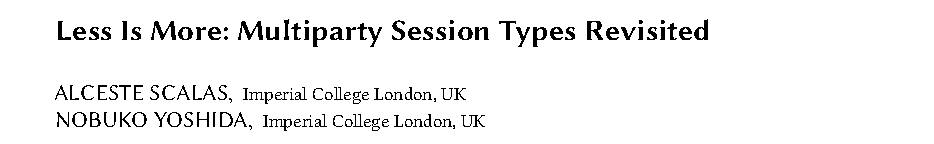
\includegraphics[width=\textwidth]{figures/less-is-more.pdf}
    \end{sticky}
    \end{minipage}

  \Put(40,40){%
    \begin{onlyenv}<2->
    \begin{minipage}{.86\columnwidth}
    \begin{sticky}
  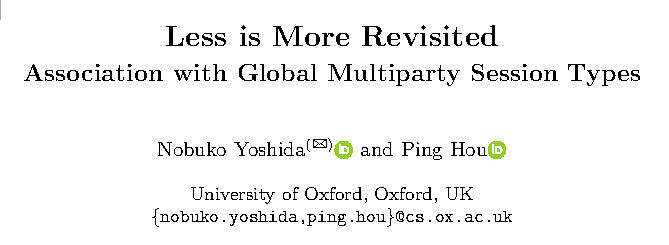
\includegraphics[width=\textwidth]{figures/less-is-more-revisite.pdf}
    \end{sticky}
    \end{minipage}
    \end{onlyenv}
   }

\end{frame}

\begin{frame}
  
\includegraphics[width=\columnwidth]{figures/xkcd-standards.png}
\end{frame}


\begin{frame}{Our Approach: Synthetic Typing}
    \begin{minipage}{.86\columnwidth}
    \begin{sticky}
  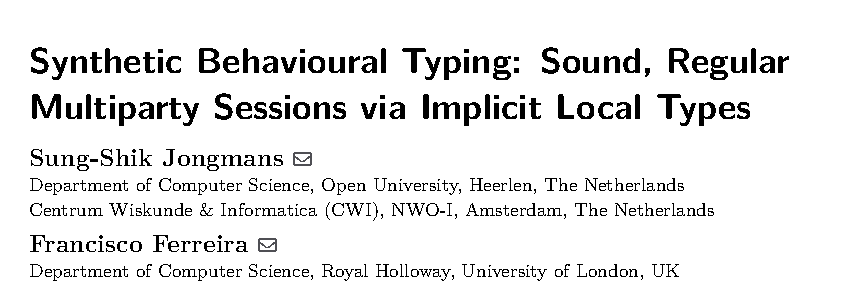
\includegraphics[width=\textwidth]{figures/fs-synthetic.pdf}
    \end{sticky}
    \end{minipage}

  \Put(40,140){%
    \begin{onlyenv}<2->
    \begin{minipage}{.86\columnwidth}
      \begin{greenbox}
        Goals:
        \begin{itemize}
          \item ``Free'' typing from being tied up to the syntax of local types.
          \item Avoid projection/merging/etc.
\item A formal description of equality
  between global types to replace informally equating global types to
  their unfolding.
          \item Well-formedness/deadlock-freedom is decided by typeability.
          \item Mechanisation in Agda.
        \end{itemize}
      \end{greenbox}
    \end{minipage}
    \end{onlyenv}
   }
\end{frame}


\begin{frame}
  \vfill
  \centering
  %\begin{beamercolorbox}[sep=8pt,center,shadow=true,rounded=true]{block}
  \begin{sticky}
    \usebeamerfont{title}
    {\normalfont \textbf{Towards Synthetic MPST (WIP)}}
    \par%
  \end{sticky}
  %\end{beamercolorbox}
  \vfill
\end{frame}

\begin{frame}{New (Synthetic) Core Typing Rules}
  \only<1>{%
  \blfootnote{Synthetic, in that $\globalt{G'}$ occurs only in the premise, not
    in the conclusion. $\globalt{G'}$ needs to be \emph{synthesised} by using
    the rules of the operational semantics of global types.}
\boxed{\textbf{New judgement}: \hspace{.2cm} $\poft \Gamma P G \Rp$}}
\vspace{.5cm}

{\scriptsize
\begin{displaymath}
  \begin{array}{c}
  \uncover<1-2>{%
  \infer[T-SEND]
  {\greduce G {\annlbl \Rp \Rq {\lbl(\expt{S})}} {G'} \and \poft \Gamma P {G'} \Rp \and
  \toft \Gamma e S}
  {\poft \Gamma {\psend \Rq \lbl e P} G \Rp}
  }

  \\[.4cm]

  \infer[T-RECV]
  {
    \only<1-4>{\forall (i \in I) \;{\text{s.t.}}\;
    \greduce G {\annlbl \Rq \Rp {\lbl_i(\expt{S_i})}} {G'}}
    \only<5>{\boxed{\forall (i \in I) \;{\text{s.t.}}\;
    \greduce G {\annlbl \Rq \Rp {\lbl_i(\expt{S_i})}} {G'}}}
    \;\text{ we have }\; \poft {\Gamma, {\pvar{x_i}} : {\expt{S_i}}} {P_i} {G'} \Rp}
  {\poft \Gamma {\precv i I {\precbr q {\lbl_i} {x_i} {P_i}}} G \Rp}

  \\[.4cm]

  \uncover<1-3>{%
  \infer[T-SKIP]
  {
    \forall (i \in I) \; \text{s.t.} \; \greduce G {\annlbl \Rq \Rp {\lbl_i(\expt{S_i})}} {G'}
    \; \text{and} \; \Rp \neq \Rr \wedge \Rq \neq \Rr
    \;\text{ we have }\;
    \poft \Gamma {P} {G'} \Rr }
  {\poft \Gamma P G \Rr}
  }
  \end{array}
\end{displaymath}
}
  \Put(40,320){%
    \begin{onlyenv}<2>
    \begin{minipage}{.86\columnwidth}
    \begin{infobox}
      \LARGE
      \textbf{What is wrong with these rules?}
    \end{infobox}
    \end{minipage}
    \end{onlyenv}
    \begin{onlyenv}<3>
    \begin{minipage}{.86\columnwidth}
    \begin{infobox}
      \LARGE
      \textbf{Hint: the problem is in these rules}
    \end{infobox}
    \end{minipage}
    \end{onlyenv}
    \begin{onlyenv}<4>
    \begin{minipage}{.86\columnwidth}
    \begin{infobox}
      \LARGE
      \textbf{Hint 2: the problem is the same in both rules, let's focus on this one}
    \end{infobox}
    \end{minipage}
    \end{onlyenv}
    \begin{onlyenv}<5>
    \begin{minipage}{.86\columnwidth}
    \begin{infobox}
      \LARGE
      \textbf{What happens if $\globalt{G}$ does not allow $\Rp$ to receive from $\Rq$?}
    \end{infobox}
    \end{minipage}
    \end{onlyenv}
  }
\end{frame}


\begin{frame}{(Hopefully) Fixed Typing Rules}
  Let $\mathcal{R}(\Rp, \Rq, \{\ell_i(\expt{S_i})\}_{i\in I},\globalt{G}) = \exists (i \in I)
  \globalt{G'}, \greduce G {\annlbl \Rp \Rq {\lbl_i(\expt{S_i})}}
             {G'}$ -- this means that an interaction between $\Rp$ and $\Rq$ is
             ``ready'' (i.e. can happen) in $\globalt{G}$.

\begin{displaymath}
  \begin{array}{@{}c@{}}
    \uncover<1,4->{%
  \infer[T-SEND]
  {\greduce G {\annlbl \Rp \Rq {\lbl(\expt{S})}} {G'} \and \poft \Gamma P {G'} \Rp \and
  \toft \Gamma e S}
  {\poft \Gamma {\psend \Rq \lbl e P} G \Rp}
  }

  \\[.4cm]

    \uncover<2,4->{%
  \infer[T-RECV]
  { \mathcal{R}(\Rq, \Rp, \{\ell_i(\expt{S_i})\}_{i \in I}, G) \and
    \forall (i \in I) \;{\text{s.t.}}\;
    \greduce G {\annlbl \Rq \Rp {\lbl_i(\expt{S_i})}} {G'}
    \;\text{ we have }\; \poft {\Gamma, {\pvar{x_i}} : {\expt{S_i}}} {P_i} {G'} \Rp}
  {\poft \Gamma {\precv i I {\precbr q {\lbl_i} {x_i} {P_i}}} G \Rp}
  }

  \\[.4cm]

    \uncover<3,4->{%
  \infer[T-SKIP]
  { \mathcal{R}(\Rq, \Rp, \{\ell_i(\expt{S_i})\}_{i \in I}, G) \wedge
    (\Rr \not\in \{\Rp, \Rq\}) \\\\
    \forall (i \in I) \; \text{s.t.} \; \greduce G {\annlbl \Rq \Rp {\lbl_i(\expt{S_i})}} {G'}
    \;\text{ we have }\;
    \poft \Gamma {P} {G'} \Rr }
  {\poft \Gamma P G \Rr}
  }
  \end{array}
\end{displaymath}
  \Put(40,290){%
    \begin{onlyenv}<5>
    \begin{minipage}{.86\columnwidth}
    \begin{greenbox}
      \begin{itemize}
        \item The rules look more complex than with a syntactic approach, but
          computing $\greduce G {\annlbl \Rq \Rp {\lbl_i(\expt{S_i})}} {G'}$ is
          entirely mechanical by using the semantics of global types.
         \item The proof of subject reduction is greatly simplified (more in a
           few slides) with this formulation.
          \item No need of projection/merging.
      \end{itemize}
    \end{greenbox}
    \end{minipage}
    \end{onlyenv}
  }
\end{frame}

\begin{frame}{Semantics}
\end{frame}

\begin{frame}{Examples}
\end{frame}

\begin{frame}{Global Type Bisimilarity}
\end{frame}

\begin{frame}{Properties of Synthetic MPST}
\end{frame}

\begin{frame}
  \vfill
  \centering
  %\begin{beamercolorbox}[sep=8pt,center,shadow=true,rounded=true]{block}
  \begin{sticky}
    \usebeamerfont{title}
    {\normalfont \textbf{Wrap Up}}

    {\normalfont\Large A Crash Course on Classic Multiparty Session Types}
    \par%
  \end{sticky}
  %\end{beamercolorbox}
  \vfill
\end{frame}

\begin{frame}{Benefits of Synthetic Typing}
\end{frame}

\begin{frame}{TODO}
\end{frame}



























































































































\endinput


\begin{frame}[fragile]
  \frametitle{Fold over Lists}

  One way to guarantee \embf{recursive functions} are \embf{well-defined} is
  via \embf{Recursion Schemes}.

  \vspace{.6cm}

  \begin{minted}{Haskell}
foldr :: (a -> b -> b) -> b -> [a] -> b
foldr g b [] = b
foldr g b (x : xs) = g x (foldr g b xs)
  \end{minted}

  \vspace{.6cm}

  There are many different kinds of Recursion Schemes (e.g. Folds,
  Paramorphisms, Unfolds, Apomorphisms, \ldots)
\end{frame}

\begin{frame}[fragile]
  \frametitle{Folds as Initial Algebras}
  \centering

  \begin{columns}
    \begin{column}{.52\textwidth}
      \begin{minted}[escapeinside=??]{Haskell}
data Fix f = In { inOp :: f (Fix f) }

fold :: Functor f =>
          (f x -> x) -> 
          Fix f -> 
          x
fold a = f
    where f (In?\tikzmark{algIni1}? x) = (a?\tikzmark{alg1}? . fmap f) x
      \end{minted}
    \end{column}
    \begin{column}{.37\textwidth}
      \begin{tikzcd}
        \mhask{f (Fix f)} \arrow[r, dotted] \arrow[d, swap, "\mhask{In}"] 
        & \mhask{f x} \arrow[d, "\mhask{a}"] 
        \\
        \mhask{Fix f}\tikzmark{algIni2} \arrow[r, dotted] 
        & \mhask{x}\tikzmark{alg2}
\end{tikzcd}
    \end{column}
  \end{columns}
  \begin{onlyenv}<2>
  \begin{tikzpicture}[overlay,remember picture,shift=(current page.south west)]
    \node[label] at (11,7.5)
    {\begin{tabular}{@{}c@{}}
      Least Fixed-Point  \\
      $\mhask{Fix f} \cong \mhask{f (Fix f)}$
    \end{tabular}}; 
  \end{tikzpicture}
  \end{onlyenv}
  \begin{onlyenv}<3>
  \begin{tikzpicture}[overlay,remember picture,shift=(current page.south west)]
    \node[label] at (10,1.5) (a) {\haskell{f}-algebra};

    \draw[overlay, golden, arrows=->, line width=.5mm]
      (a) -- (pic cs:alg1);
    \draw[overlay, golden, arrows=->, line width=.5mm]
      (a) -- ($(pic cs:alg2) + (-.1, -.2)$);
  \end{tikzpicture}
  \end{onlyenv}
  \begin{onlyenv}<4>
  \begin{tikzpicture}[overlay,remember picture,shift=(current page.south west)]
    \node[label] at (7,1.5) (a)
      {initial \haskell{f}-algebra}; 

    \draw[overlay, golden, arrows=->, line width=.5mm]
      (a) -- (pic cs:algIni1);
    \draw[overlay, golden, arrows=->, line width=.5mm]
      (a) -- ($(pic cs:algIni2) + (-.8, -.2)$);
  \end{tikzpicture}
  \end{onlyenv}
\end{frame}

\begin{frame}[fragile]
  \frametitle{Folds as Initial Algebras: Lists}
    \begin{minipage}{.86\columnwidth}
    \begin{greenbox}
      \small
      \begin{haskellcode}
data ListF a b = NilF | ConsF a b
type List a = Fix (ListF a)

foldAlg :: (a -> b -> b) -> b -> ListF a b -> b
foldAlg _ z NilF        = z
foldAlg f _ (ConsF a b) = f a b

foldr :: (a -> b -> b) -> b -> List a -> b
foldr f z = fold (foldAlg f z)
      \end{haskellcode}
    \end{greenbox}
    \end{minipage}
\end{frame}


\begin{frame}[fragile]
  \frametitle{Hylomorphisms: Divide-and-conquer Recursion}
  \centering
  
  \begin{columns}
    \begin{column}{.52\textwidth}
      \begin{minted}[escapeinside=??]{Haskell}
hylo :: Functor f =>
          (f b -> b) -> 
          (a -> f a) -> 
          a -> b
hylo a c = a ?\tikzmark{halg1}? . fmap (hylo a c) . c ?\tikzmark{hcoalg1}?
      \end{minted}
    \end{column}
    \begin{column}{.37\textwidth}
      \begin{tikzcd}
        \mhask{f a} \arrow[r, dotted] 
        & \mhask{f b} \arrow[d, "\mhask{a}"] 
        \\
        \mhask{a}\tikzmark{hcoalg2} \arrow[u, "\mhask{c}"] \arrow[r, dotted] 
        & \mhask{b}\tikzmark{halg2}
\end{tikzcd}
    \end{column}
  \end{columns}

  \begin{onlyenv}<3>
  \begin{tikzpicture}[overlay,remember picture]
    \node[label] at (2,-1) (ha)
      {\begin{tabular}{@{}c@{}}
        \haskell{f}-algebra \\
        ``conquer''
      \end{tabular}}; 

    \draw[overlay, golden, arrows=->, line width=.5mm]
      (ha) -- (pic cs:halg1);
    \draw[overlay, golden, arrows=->, line width=.5mm]
      (ha) -- ($(pic cs:halg2) + (-.1, -.2)$);
  \end{tikzpicture}
  \end{onlyenv}

  \begin{onlyenv}<2>
  \begin{tikzpicture}[overlay,remember picture]
    \node[label] at (9,-1) (hc)
      {\begin{tabular}{@{}c@{}}
        \haskell{f}-coalgebra \\
        ``divide''
      \end{tabular}}; 

    \draw[overlay, golden, arrows=->, line width=.5mm]
      (hc) -- (pic cs:hcoalg1);
    \draw[overlay, golden, arrows=->, line width=.5mm]
      (hc) -- ($(pic cs:hcoalg2) + (-.1, -.2)$);
  \end{tikzpicture}
  \end{onlyenv}
\end{frame}

\begin{frame}[fragile]
  \frametitle{Folds as Hylomorphisms}
  \centering
  
  \begin{columns}
    \begin{column}{.52\textwidth}
      \begin{minted}[escapeinside=??]{Haskell}
data Fix f = In { inOp :: f (Fix f) }

fold :: Functor f =>
          (f x -> x) -> 
          Fix f -> 
          x
fold a = a?\tikzmark{fhalg1}? . fmap (fold a) . inOp?\tikzmark{fhcoalg1}?
      \end{minted}
    \end{column}
    \begin{column}{.37\textwidth}
      \begin{tikzcd}
        \tikzmark{fhcoalg2}\mhask{f (Fix f)} \arrow[r, dotted] 
        & \mhask{f x} \arrow[d, "\mhask{a}"] 
        \\
        \mhask{Fix f} \arrow[u, "\mhask{inOp}"] \arrow[r, dotted] 
        & \mhask{x}\tikzmark{fhalg2}
\end{tikzcd}
    \end{column}
  \end{columns}

  \begin{tikzpicture}[overlay,remember picture]
    \node[label] at (2,-1) (fha)
      {\haskell{f}-algebra}; 

    \draw[overlay, golden, arrows=->, line width=.5mm]
      (fha) -- ($(pic cs:fhalg1) + (.2, 0)$);
    \draw[overlay, golden, arrows=->, line width=.5mm]
      (fha) -- ($(pic cs:fhalg2) + (-.1, -.2)$);
  \end{tikzpicture}

  \begin{tikzpicture}[overlay,remember picture]
    \node[label] at (9,5) (fhc)
      {\haskell{f}-coalgebra}; 

    \draw[overlay, golden, arrows=->, line width=.5mm]
      (fhc) -- ($(pic cs:fhcoalg1) + (-.2, .3)$);
    \draw[overlay, golden, arrows=->, line width=.5mm]
      (fhc) -- ($(pic cs:fhcoalg2) + (.7, .4)$);
  \end{tikzpicture}
\end{frame}

\begin{frame}[fragile]
  \frametitle{Example: Nonstructural Recursion}
  \centering

  \begin{columns}
    \begin{column}{.38\textwidth}
      \begin{minted}[escapeinside=??, fontsize=\scriptsize]{Haskell}
data TreeC a b = Leaf |  Node b a b

split [] = Leaf?\tikzmark{qscoalg1}?
split (h : t) = Node l h r
  where
    (l, r) = partition (\x -> x < h) t

merge Leaf = \acc -> acc
merge (Node l x r) = \acc -> l (x : r acc)?\tikzmark{qsalg1}?
      \end{minted}
    \end{column}
    \begin{column}{.59\textwidth}\scriptsize
      \begin{tikzcd}[nodes={column sep=5em}]
        \tikzmark{qscoalg2}\mhask{TreeC Int [Int]} \arrow[r, dotted, "\mhask{fmap qsort}"]
        & \mhask{TreeC Int ([Int] -> [Int])} \arrow[d, "\mhask{merge}"]
        \\
        \mhask{[Int]} \arrow[u, "\mhask{split}"] \arrow[r, dotted, "\mhask{qsort}"] 
        & \mhask{[Int] -> [Int]}\tikzmark{qsalg2}
\end{tikzcd}
    \end{column}
  \end{columns}

  \begin{overprint}
    \onslide<2>
  \begin{tikzpicture}[overlay,remember picture,shift=(current page.south west)]
    \node[label] at (12,2) (qsa)
      {\haskell{TreeC Int}-algebra};

    \draw[overlay, golden, arrows=->, line width=.5mm]
      (qsa) -- ($(pic cs:qsalg1) + (.2, 0)$);
    \draw[overlay, golden, arrows=->, line width=.5mm]
      (qsa) -- ($(pic cs:qsalg2) + (-1, -.2)$);
  \end{tikzpicture}

  \begin{tikzpicture}[overlay,remember picture,shift=(current page.south west)]
    \node[label] at (10,7) (qsc)
      {\haskell{TreeC Int}-coalgebra};

    \draw[overlay, golden, arrows=->, line width=.5mm]
      (qsc) -- ($(pic cs:qscoalg1) + (.2, .3)$);
    \draw[overlay, golden, arrows=->, line width=.5mm]
      (qsc) -- ($(pic cs:qscoalg2) + (1, .4)$);
  \end{tikzpicture}
  \end{overprint}
\end{frame}

% \begin{frame}[fragile]
%   \frametitle{Adjoint Folds}
%   Given an adjunction:
% 
%   \begin{center}\LARGE
%   \begin{tikzcd}
%     \mathcal{D} \arrow[r, swap, "\mathsf{R}"{name=G}, bend right=25] &
%     \mathcal{C} \arrow[l, swap, "\mathsf{L}"{name=F}, bend right=25]
%     \arrow[phantom, from=F, to=G, "\dashv" rotate=-90]
%   \end{tikzcd}
%   \end{center}
% 
%  \begin{itemize}
%    \item There is a correspondence of arrows 
%      $\lfloor\cdot\rfloor : \mathsf{Hom}_{\mathcal{D}}(L\, A,B) \cong 
%      \mathsf{Hom}_{\mathcal{C}}(A,R\, B) : \lceil\cdot\rceil$.
%    \item An initial algebra on the right corresponds to an universal property
%      on the left:
%      {\large
%      \[
%        \mathsf{Hom}_{\mathcal{D}}(L\, \mu F, B) \cong \mathsf{Hom}_{\mathcal{C}}(\mu F,R\, B)
%      \]}\blfootnote{$\mu$ analogous to Haskell's \haskell{Fix}}\blfootnote{$F$
%      is an endofunctor in $\mathcal{C}$}\blfootnote{$L$, $R$ are functors
%      between $\mathcal{C}$ \& $\mathcal{D}$; the \emph{left} and \emph{right}
%      adjoints.}
%  \end{itemize}
% \end{frame}
%  %\arrow[phantom, from=F, to=G, "\dashv" rotate=-90, no line]

% NOTES:
% - Every complex recursion scheme is an hylomorphism via its associated
%   adjunction/conjugate pair 

% - (e.g) folds with parameters (accumulators) use the curry/uncurry adjunction 

% - a recursion scheme from comonads (RSFCs, Uustalu, Vene, Pardo, 2001) is an conjugate hylomorphism via the coEilemberg-Moore category for the cofree comonad.
\begin{frame}[fragile]
  \frametitle{Conjugate Hylomorphisms}
  \centering
  {\Large\emph{Every recursion scheme is a conjugate hylomorphism}}%
  \blfootnote{\tiny{}R. Hinze, N. Wu, J. Gibbons: \textbf{Conjugate
  Hylomorphisms - Or: The Mother of All Structured Recursion Schemes}. POPL
  2015.}

  \vspace{.4cm}

  \begin{sticky}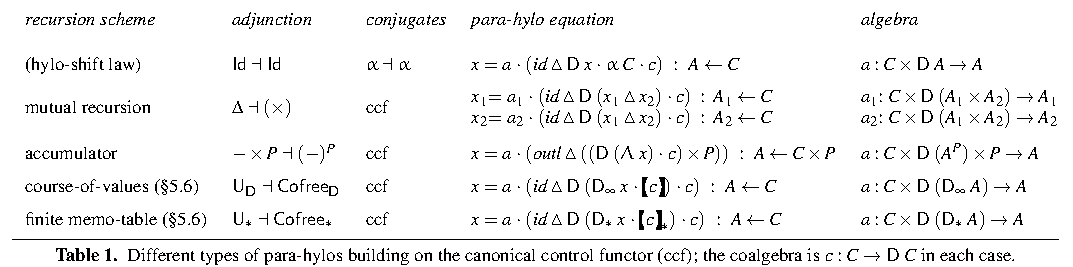
\includegraphics[width=\textwidth]{figures/types-of-parahylos-crop.pdf}\end{sticky}

  \Put(40,290){%
    \begin{onlyenv}<2>
    \begin{minipage}{.86\columnwidth}
    \begin{greenbox}
      \small
      \begin{itemize}
        \item Every complex recursion scheme is a hylomorphism via its associated adjunction/conjugate pair
        \item (e.g) Folds with parameters (accumulators) use the curry/uncurry adjunction
        \item A recursion scheme from comonads (RSFCs, Uustalu, Vene, Pardo, 2001) is an conjugate hylomorphism via the coEilenberg-Moore category for the cofree comonad
      \end{itemize}
    \end{greenbox}
    \end{minipage}
    \end{onlyenv}
  }
\end{frame}

\begin{frame}
  \frametitle{Why Mechanising Hylomorphisms in Coq?}

  \begin{itemize}
    \item Structured Recursion Schemes have been used in Haskell to structure
      functional programs, but they do not ensure termination/productivity
    \item On the other hand, Coq does not capture all recursive definitions
    \item The benefits of formalising hylos in Coq is three fold:
      \begin{itemize}
        \item Giving the Coq programmer a \embf{library} where for most
          recursion schemes they do not have to prove termination properties
        \item \embf{Extracting code} into ML/Haskell to provide termination
          guarantees even in languages with non-termination
        \item Using the laws of hylomorphisms as tactics for \embf{program
          calculation} and \embf{optimisation}
      \end{itemize}
  \end{itemize}
\end{frame}

\begin{frame}
  \frametitle{Challenges}
  \begin{enumerate}
    \item Avoiding axioms: functional extensionality, heterogeneous equality,
      \ldots.
    \item Extracting ``clean'' code: close to what a programmer would have
      written directly in OCaml.
    \item Fixed-points of functors, non-termination, etc.
  \end{enumerate}

  \vspace{.5cm}
  
  \uncover<2->{%
    Our solutions (the remainder of this talk):
    \begin{enumerate}
      \item<2-> Machinery for building setoids, use of decidable predicates, \ldots
      \item<3-> Avoiding type families and indexed types.
      \item<4-> \embf{Containers} \& \embf{recursive coalgebras}
    \end{enumerate}
   }

\end{frame}


\begin{frame}
  \frametitle{Roadmap}
  \centering
  \LARGE

    \begin{sticky}%
      \vspace{-1.5em}
      \begin{tabular}{@{}rl}
        {\textbf{\color{gray}Part I:}} & Extractable Containers in Coq \\
        {\textbf{\color{gray}Part II:}} & Recursive Coalgebras \& Coq Hylomorphisms \\
        {\textbf{\color{gray}Part III:}} & Code Extraction \& Examples 
      \end{tabular}
    \end{sticky}
\end{frame}
% 
% \begin{frame}
%   \frametitle{Why Mechanising Hylomorphisms in Coq?}
% 
%   \begin{itemize}
%   \end{itemize}
% \end{frame}
% 
\begin{frame}
  \vfill
  \centering
  %\begin{beamercolorbox}[sep=8pt,center,shadow=true,rounded=true]{block}
  \begin{sticky}
    \usebeamerfont{title}
    {\normalfont Part I}

    {\normalfont\Large Extractable Containers in Coq}
    \par%
  \end{sticky}
  %\end{beamercolorbox}
  \vfill
\end{frame}

\begin{frame}
  \frametitle{Containers}

  Containers are defined by a  pair $S \triangleleft P$:\blfootnote{%
    Abbott, Altenkirch, Ghani: \textbf{Categories of Containers}. FoSSaCS 2003.
  }
  \begin{itemize}
    \item a type of \alert{shapes} $S : \mathsf{Type}$
    \item a \alert{family} of positions, indexed by shape $P : S \to \mathsf{Type}$
  \end{itemize}

  \vspace{.7cm}
  \uncover<2>{%
    A \alert{container extension} is a functor defined as follows
    \[
      \begin{array}{ll}
        \llbracket S \triangleleft P \rrbracket\; X & = \Sigma_{s : S} P\;s \to X \\[.3cm]
      \llbracket S \triangleleft P \rrbracket\; f & = \lambda (s, p). \; (s, f \circ p)
      \end{array}
    \]
  }
\end{frame}

\begin{frame}
  \frametitle{Example}

  Consider the functor
  \only<1>{$F\; X = \mathcolorbox{white}{1} + \mathcolorbox{white}{X\times X}$}%
  \only<2>{$F\; X = \mathcolorbox{golden}{1} + \mathcolorbox{golden}{X\times X}$}%
  \only<3>{$F\; X = \mathcolorbox{golden}{1} + \mathcolorbox{white}{X\times X}$}%
  \only<4>{$F\; X = \mathcolorbox{white}{1} + \mathcolorbox{golden}{X\times X}$}%
  \vspace{.2cm}

  $S_{F}$ and $P_{F}$ define a container that is isomorphic to $F$

  \[
    \only<1>{S_F = \mathcolorbox{white}{1} + \mathcolorbox{white}{1}}%
    \only<2>{S_F = \mathcolorbox{golden}{1} + \mathcolorbox{golden}{1}}%
    \only<3>{S_F = \mathcolorbox{golden}{1} + \mathcolorbox{white}{1}}%
    \only<4>{S_F = \mathcolorbox{white}{1} + \mathcolorbox{golden}{1}}%
    \tikzmark{shapeC}
    \hspace{.5cm}
      \begin{array}{l}
        \only<1-2,4->{\mathcolorbox{white}{P_{F}\;(\mathsf{inl}\;\sbullet) = 0}}%
        \only<3>{\mathcolorbox{golden}{P_{F}\;(\mathsf{inl}\;\sbullet) = 0}}%
        \tikzmark{pos0}
        \\
        \only<1-3>{\mathcolorbox{white}{P_{F}\;(\mathsf{inr}\;\sbullet) = 1+1}}%
        \only<4>{\mathcolorbox{golden}{P_{F}\;(\mathsf{inr}\;\sbullet) = 1+1}}%
        \tikzmark{pos1}
      \end{array}
   \]
   \vspace{.4cm}

  Examples of objects of types $F\;\mathbb{N}$ (left) and
$\llbracket S_F \triangleleft P_F \rrbracket\;\mathbb{N}$ (right):
   \[\begin{array}{r c l}
        \mathsf{inl}\;\sbullet & \cong & (\mathsf{inl}\;\sbullet, !_{\mathbb{N}})
      \\
        \mathsf{inr}\;(7,9) & \cong &
        (\mathsf{inr}\;\sbullet, \lambda x, \mathsf{case}\;x\;\{%
          \begin{array}{l}
            \mathsf{inl}\;\sbullet \Rightarrow 7;\;\;
            \mathsf{inr}\;\sbullet \Rightarrow 9
          \end{array}
          \})
      \end{array}
  \]

  \begin{overprint}
    \onslide<2>
  \begin{tikzpicture}[overlay,remember picture,shift=(current page.south west)]
    \node[label] at (12,7) (cos)
      {Two cases (``shapes'')};
  \end{tikzpicture}
  \end{overprint}
  \begin{overprint}\onslide<3>
  \begin{tikzpicture}[overlay,remember picture,shift=(current page.south west)]
    \node[label] at (10,8) (copl)
      {No positions on the left shape};
  \end{tikzpicture}
  \end{overprint}
  \begin{overprint}\onslide<4>
  \begin{tikzpicture}[overlay,remember picture,shift=(current page.south west)]
    \node[label] at (10,8) (copl)
      {Two positions on the right shape};
  \end{tikzpicture}
  \end{overprint}
\end{frame}

\begin{frame}[fragile]
  \frametitle{Mechanising Containers: Setoids and Morphisms}
  To avoid the functional extensionality axiom, we use:
  \begin{itemize}
    \item \embf{setoids}: types with an associated equivalence
    \item \embf{proper morphisms} of the respectfulness relation: functions
      that map related inputs to related outputs
  \end{itemize}
  \vspace{.6cm}
  \begin{tabular}{@{}rl@{}}
    \alert{Setoids:} & Given \colorbox{lime}{\coq{setoid A}}, and
  \colorbox{lime}{\coq{x y : A}}, we write 
  \colorbox{lime}{\coq{x =e y : Prop}}.
    \\[.5cm]
    \alert{Morphisms}: & Given 
  \colorbox{lime}{\coq{setoid A}} and 
  \colorbox{lime}{\coq{setoid B}}, we write
  \colorbox{lime}{\coq{f : A ~> B}}.
  \end{tabular}

  \Put(30,160){%
    \begin{onlyenv}<2>
    \begin{minipage}{.86\columnwidth}
    \begin{greenbox}
      \small
      \begin{itemize}
        \item We provide automatic coercion from \coq{A ~> B} to \coq{A -> B}.
        \item Coq's extraction mechanism ignores the \coq{Prop} field.
        \item We provide a (very basic!) mechanism to help building morphisms.
        \item Building on top of setoids \& morphisms allows the  use of Coq's
\alert{generalised rewriting}.
      \end{itemize}
    \end{greenbox}
    \end{minipage}
    \end{onlyenv}
  }
\end{frame}

\begin{frame}[fragile]
  \frametitle{Containers in Coq: A Bad Attempt}
  Assume a \coq{Shape : Type} and \coq{Pos : Shape -> Type}.
  \vspace{.4cm}

  We can define a container extension in the straightforward way:
  \begin{minted}{coq}
Record App (X : Type) :=
  MkCont { shape : Shape; contents : Pos shape -> X }.
  \end{minted}
  \vspace{.2cm}

  \begin{overprint}
    \onslide<2->
  \begin{center}
  \begin{minipage}{.8\columnwidth}
    \begin{infobox}
      \begin{itemize}
        \item The above definition forces us to use dependent equality and
          UIP/Axiom K/\ldots E.g.: dealing with  \coq{eq_dep s1 p1 s2 p2} if
          \coq{p1 : Pos s1} and \coq{p2 : Pos s2}.
        \item Type families lead to OCaml code with \ocaml{Obj.magic}.
      \end{itemize}
    \end{infobox}
  \end{minipage}
  \end{center}
  \end{overprint}
\end{frame}

\begin{frame}[fragile]
  \frametitle{Extractable Containers in Coq (I)}

  Observations:
  \begin{enumerate}
    \item UIP is \alert{not an axiom} in Coq for types with a \alert{decidable
      equality}.
    \item If a type family is defined as a \alert{predicate subtype}, Coq can
      erase the predicate and extract code that is equivalent to the supertype.
      E.g. \coq{{x | P x}} for some \coq{P : X -> Prop}.
  \end{enumerate}
\end{frame}

\begin{frame}[fragile]
  \frametitle{Extractable Containers in Coq (and II)}
  Our containers are defined by:
  \begin{itemize}
    \item \coq{Sh : Type}: type of shapes
    \item \coq{Po : Type}: type of \alert{all} positions
    \item \coq{valid : Sh * Po ~> bool}
      \begin{itemize}
        \item[] \alert{decidable} predicate stating when a pair shape/position is valid
      \end{itemize}
  \end{itemize}
  \vspace{.6cm}

  Container extensions that lead to ``clean'' code extraction:
  \begin{coqcode}
    Record App (X : Type)
    := MkCont { shape : Sh;
                contents : {p | valid (shape, p)} -> X
              }.
  \end{coqcode}
  \Put(40,290){%
    \begin{onlyenv}<2>
    \begin{minipage}{.86\columnwidth}
    \begin{greenbox}
      \small
      \begin{itemize}
        \item All proofs of the form \coq{V1 V2 : valid(s,p) = true} are
              provably equal in Coq to \coq{eq_refl}.
        \item Given \coq{p1 p2 : {p | valid(s, p)}}, \coq{p1 = p2} iff \coq{proj1_sig p1 = proj1_sig p2}.
        \item Extraction will treat the contents of container extensions equivalently to
              \coq{contents : Po -> X}
              \item[] (\ul{no unsafe coercions}).
      \end{itemize}
    \end{greenbox}
    \end{minipage}
    \end{onlyenv}
  }
\end{frame}

\begin{frame}[fragile]
  \frametitle{Example: $F\; X = 1 + X \times X$}

\begin{onlyenv}<1>
  Container definition:
  \vspace{.2cm}

\begin{coqcode}
Inductive ShapeF := Lbranch | Rbranch.
Inductive PosF := Lpos | Rpos.

Definition validF (x : ShapeF * PosF) : bool
  := match fst x with | Lbranch => false | Rbranch => true end.
\end{coqcode}
\end{onlyenv}
\begin{onlyenv}<2>
  Example object equivalent to $\mathsf{inr}\;(7,8)$
  \vspace{.2cm}

\begin{coqcode}
Example e1 : App nat :=
  MkCont Rbranch (fun p => match elem p with
                           | Lpos => 7 | Rpos => 8
                           end).
\end{coqcode}
\end{onlyenv}
\end{frame}

%\begin{frame}
%  \frametitle{Container Equality}
%\end{frame}


\begin{frame}
  The argument of container extensions occurs in \ul{strictly positive} positions:
  \begin{itemize}
    \item[] We can define \ul{least/greatest fixed points of container extensions}.
  \end{itemize}
  \vspace{.5cm}

  We provide a library of polynomial functors as containers, as well as custom
  shapes (e.g. binary trees) that we use in our examples.
  \vspace{.5cm}

  \vspace{.5cm}
  \textbf{Not discussed:}
  \begin{itemize}
    \item Container morphisms and \ul{natural transformations}
    \item Container composition $S \triangleleft P = (S_1 \triangleleft P_1) \circ (S_2 \triangleleft P_2)$
    \item Container equality
  \end{itemize}

\end{frame}

\begin{frame}
  \vfill
  \centering
  %\begin{beamercolorbox}[sep=8pt,center,shadow=true,rounded=true]{block}
  \begin{sticky}
    \usebeamerfont{title}
    {\normalfont Part II}

    {\normalfont\Large Recursive Coalgebras \& Coq Hylomorphisms}
    \par%
  \end{sticky}
  %\end{beamercolorbox}
  \vfill
\end{frame}

\begin{frame}[fragile]
  \frametitle{Algebras \& Container Initial Algebras}

  The least fixed-point of a container extension \coq{App C} is:
  \begin{coqcode}
    Inductive LFix C := Lin { lin_op : App C (LFix C) }.
  \end{coqcode}
  \vspace{.4cm}

  Algebras are of type \coq{Alg C X = App C X ~> X}.
  \vspace{.4cm}

  \textbf{Catamorphisms:}
  \begin{coqcode}
cata : Alg C X ~> LFix C ~> X

cata_univ : forall (a : Alg C X) (f : LFix C ~> X),
  f \o Lin =e a \o fmap f <-> f =e cata a
  \end{coqcode}
\end{frame}

\begin{frame}[fragile]
  \frametitle{Coalgebras \& Container Terminal Coalgebras}

  The \ul{greatest} fixed-point of a container extension \coq{App C} is:
  \begin{coqcode}
    CoInductive GFix C := Gin { gin_op : App C (GFix C) }.
  \end{coqcode}
  \vspace{.4cm}

  Coalgebras are of type \coq{CoAlg C X = X ~> App C X}.
  \vspace{.4cm}

  \textbf{Anamorphisms:}
  \begin{coqcode}
ana : CoAlg C X ~> X ~> GFix C

ana_univ : forall (c : CoAlg C X) (f : X ~> GFix C),
  gin_op \o f =e fmap f \o c <-> f =e ana c
  \end{coqcode}
\end{frame}

\begin{frame}[fragile]
  \frametitle{Recursive Coalgebras (I)}

  We cannot define \coq{hylo} in Coq using arbitrary coalgebras, because they may not exist...

  \uncover<2->{But they exist for \textbf{recursive coalgebras}.%
    \blfootnote{J. Adámek, S. Milius, L.S. Moss:
\textbf{On Well-Founded and Recursive Coalgebras}. FoSSaCS 2020.}
  }
  \vspace{.6cm}

  \uncover<3->{%
    \textbf{Recursive coalgebras}: coalgebras (\coq{c : CoAlg C X}) that terminate in all inputs.
    \begin{itemize}
      \item<3-> i.e. their anamorphisms only produce \ul{finite trees}.
      \item<4-> i.e. they decompose inputs into ``smaller'' values of type \coq{X}
    \end{itemize}
  }
\end{frame}

\begin{frame}
  \frametitle{Recursive Coalgebras (and II)}

  We define a predicate \coq{RecF c x} that states that \coq{c : CoAlg C X}
terminates on \coq{x : X}.
     \vspace{.4cm}

  Using \coq{RecF}, we define:
    \begin{enumerate}
      \item Recursive coalgebras:

            \coq{RCoAlg C X = {c | forall x, RecF c x}}

      \item Given a well-founded relation \coq{R}, well-founded coalgebras

            \coq{WfCoalg C X = {c | forall x p, R (contents (c x) p) x}}
     \end{enumerate}
     \vspace{.4cm}

    \begin{itemize}
    \item<2-> Definitions (1) and (2) are equivalent
    \item<3-> Our mechanisation represents (2) in terms of (1)
    \item<4-> Termination proofs may be easier using (1) or (2), depending on the
use case
    \end{itemize}
\end{frame}

\begin{frame}[fragile]
  \frametitle{Recursive Hylomorphisms}

  \textbf{Recall:}
\vspace{.2cm}

  Hylomorphisms are solutions to the equation
$f = a \circ \mathsf{fmap}\;f \circ c$.

\vspace{.2cm}
  Due to termination, this solution \ul{may not exist}, or \ul{may not be unique}.

\vspace{.2cm}
  If $c$ is recursive, then the solution \textbf{is unique, and guaranteed to exist}.
\vspace{.4cm}

  \begin{overprint}
    \onslide<2->
    \begin{minipage}{\textwidth}
      \begin{bluebox}
      \begin{coqcode}
Definition hylo_def (a : Alg F B) (c : Coalg F A)
  : forall (x : A), RecF c x -> B :=
  fix f x H :=
    match c x as cx
          return (forall e : Pos (shape cx), RecF c (cont cx e)) -> B
    with
    | MkCont sx cx => fun H => a (MkCont sx (fun e => f (cx e) (H e)))
    end (RecF_inv H).
      \end{coqcode}
      \end{bluebox}
    \end{minipage}
  \end{overprint}

\end{frame}

\begin{frame}[fragile]
  \frametitle{Universal Property of Recursive Hylomorphisms}

  We define wrappers over \coq{hylo_def}:
  \vspace{.2cm}

  \begin{center}
  \begin{minipage}{.6\textwidth}
  \begin{bluebox}
  \begin{coqcode}
hylo : Alg C B ~> RCoAlg C A ~> A ~> B
  \end{coqcode}
  \end{bluebox}
  \end{minipage}
  \end{center}

  \vspace{.6cm}
  From this definition, we can prove the universal property of hylomorphisms.

  Given \coq{a : Alg C B} and \coq{c : RCoAlg C A}:
  \vspace{.2cm}

  \begin{center}
  \begin{minipage}{.6\textwidth}
  \begin{bluebox}
  \begin{coqcode}
hylo_univ : forall f : A ~> B,
  f =e a \o fmap f \o c <-> f = hylo a c
  \end{coqcode}
  \end{bluebox}
  \end{minipage}
  \end{center}

\end{frame}

\begin{frame}[fragile]
  \frametitle{A Note on Recursive Anamorphisms}

  For simplicity, we define \ul{recursive anamorphisms} as
  \coq{rana c = hylo Lin c}.
  \begin{itemize}
  \item This way we avoid the need to convert \coq{GFix} to \coq{LFix}.
  \item We prove (straightforward) that \coq{rana c} is equal to \coq{ana c},
followed by converting the result to \coq{LFix}.
  \end{itemize}

\end{frame}

\begin{frame}[t,fragile]
  \frametitle{Proving the Laws of Hylomorphisms}

The following \coq{hylo_fusion} laws \ul{are straightforward consequences} of
\coq{hylo_univ}.\only<2>{%
  \blfootnote{\tiny{}R. Hinze, N. Wu, J. Gibbons: \textbf{Conjugate
  Hylomorphisms - Or: The Mother of All Structured Recursion Schemes}. POPL
  2015.}
  }
\vspace{.2cm}

  \begin{center}
  \begin{minipage}{.82\textwidth}
  \begin{bluebox}
  \begin{coqcode}
Lemma hylo_fusion_l
    : h \o a =e b \o fmap h -> h \o hylo a c =e hylo b c.

Lemma hylo_fusion_r
    : c \o h =e fmap h \o d -> hylo a c \o h =e hylo a d.

Lemma deforest : cata a \o rana c =e hylo a c.
  \end{coqcode}
  \end{bluebox}
  \end{minipage}
  \end{center}


  \Put(40,90){%
    \begin{onlyenv}<2>
    \begin{minipage}{.86\columnwidth}
      \small
    \begin{greenbox}
      The \ul{proofs in Coq are almost direct copies from pen-and-paper proofs}:
By \coq{hylo_univ}, \coq{hylo b c} is the only arrow making the outer square
commute.
\[\begin{tikzcd}[ampersand replacement=\&, nodes={column sep=5.5em}]
	{t b} \& { ta} \& {tc} \\
	{f\; tb} \& {f\;ta} \& {f\;tc}
	\arrow["h"', from=1-2, to=1-1]
	\arrow["\mathsf{hylo}\;a\;c"', from=1-3, to=1-2]
	\arrow["c", from=1-3, to=2-3]
	\arrow["b", from=2-1, to=1-1]
	\arrow["a", from=2-2, to=1-2]
	\arrow["{\mathsf{fmap}\;h}", from=2-2, to=2-1]
	\arrow["{\mathsf{fmap}\;(\mathsf{hylo}\;a\;c)}", from=2-3, to=2-2]
\end{tikzcd}\]
    \end{greenbox}
    \end{minipage}
    \end{onlyenv}
  }

\end{frame}

\begin{frame}[fragile]
  \begin{center}
    \begin{itemize}
    \item Our formalisation allows to do equational reasoning that closely
mirrors pen-and-paper proofs.
    \item \coq{hylo_fusion} can be applied to \emph{calculate} optimised
programs by fusing simpler specifications in Coq.
    \item This leads to more modular development and proofs, without affecting
the performance of the extracted code.
    \end{itemize}
  \end{center}
\end{frame}

\begin{frame}
  \vfill
  \centering
  %\begin{beamercolorbox}[sep=8pt,center,shadow=true,rounded=true]{block}
  \begin{sticky}
    \usebeamerfont{title}
    {\normalfont Part III}

    {\normalfont\Large Code Extraction \& Examples}
    \par%
  \end{sticky}
  %\end{beamercolorbox}
  \vfill
\end{frame}

\begin{frame}[fragile]
  \frametitle{A Tree Container for Divide \&Conquer}

  Our divide-and-conquer examples use a tree container \coq{TreeC A B} that is
isomorphic to:
  \[
    T\; A\; B\; X = A + B \times X \times X
  \]
  \vspace{.3cm}

  Given two setoids \coq{A} and \coq{B}, we define the following wrappers in
Coq:
\vspace{.4cm}

\begin{center}
\begin{minipage}{.65\textwidth}
\begin{bluebox}
  \begin{coqcode}
a_node : B ~> X ~> X ~> App (TreeC A B) X
a_leaf : A ~> App (TreeC A B) X
a_out : App (TreeC A B) X ~> A + B * X * X
  \end{coqcode}
\end{bluebox}
\end{minipage}
\end{center}
\end{frame}

\begin{frame}[fragile]
  \frametitle{Quicksort Definition}

  \begin{coqcode}
Definition mergeF (x : App (TreeC unit int) (list int)) : list int :=
  match a_out x with
  | inl _ => nil
  | inr (p, l, r) => List.app l (h :: r)
  end.

Definition splitF (l : list int) : App (TreeC unit int) (list int) :=
  match x with
  | nil => a_leaf tt
  | cons h t => let (l, r) := List.partition (fun x => x <=? h) t in
                a_node h l r
  end.
  \end{coqcode}
\end{frame}

\begin{frame}[fragile]
  \frametitle{Quicksort Extraction}
    \begin{minipage}{.86\columnwidth}
    \begin{bluebox}
    \begin{coqcode}
Definition qsort := hylo merge split.
Extraction qsort.
    \end{coqcode}
    \end{bluebox}
    \end{minipage}

  \vspace{.6cm}

    \begin{overprint}
    \onslide<2->
    \begin{minipage}{.86\columnwidth}
    \begin{greenbox}
    \begin{ocamlcode}
let rec qsort = function
| [] -> []
| h :: t ->
  let (l, r) = partition (fun x0 -> leb x0 h) t in
  let x0 = fun e -> qsort (match e with
                           | Lbranch -> l
                           | Rbranch -> r) in
  app (x0 Lbranch) (h :: (x0 Rbranch))
    \end{ocamlcode}
    \end{greenbox}
    \end{minipage}
    \end{overprint}
\end{frame}

\begin{frame}[fragile]
  \frametitle{Using Hylo-fusion for Program Optimisation}

  \begin{onlyenv}<1>
    \begin{minipage}{.86\columnwidth}
    \begin{bluebox}
    \begin{coqcode}
Definition qsort_times_two
  : {f | f =e map times_two \o hylo merge split}.
  eapply exist.
  (* ... *)
  rewrite (hylo_fusion_l H); reflexivity.
Defined.

Extraction qsort_times_two.
    \end{coqcode}
    \end{bluebox}
    \end{minipage}
  \end{onlyenv}

  \begin{onlyenv}<2>
    \begin{minipage}{.92\columnwidth}
    \begin{greenbox}
    \begin{ocamlcode}
let rec qsort_times_two = function
| [] -> []
| h :: t ->
  let (l, r) = partition (fun x0 -> leb x0 h) t in
  let x0 = fun p -> qsort_times_two (match p with
                                     | Lbranch -> l
                                     | Rbranch -> r) in
  app (x0 Lbranch) ((mul (Uint63.of_int (2)) h) :: (x0 Rbranch))
    \end{ocamlcode}
    \end{greenbox}
    \end{minipage}
    \end{onlyenv}
\end{frame}

\begin{frame}
  \frametitle{A Recursion Scheme for Dynamic Programming}
  Given a functor $G$, we can construct a
  memoisation table $G_{\ast} A = \mu X. A \times G X$.

  We can index the memoisation table, extract its head, and insert a new element:
  \[
    \begin{array}{@{}l@{}}
      \mathsf{look} : \mathbb{N} \times G_{{\ast}}A \to 1 + A \hspace{.5cm}
      \mathsf{head} : G_{\ast} A \to A \hspace{.5cm}
      \mathsf{Cons} : A \times G (G_{\ast} A) \to G_{\ast} A
    \end{array}
  \]

  \vspace{.2cm}
  Given an algebra $a : G(G_{\ast}A)\to A$, we can construct
  \[ a'= \mathsf{Cons} \circ \mathsf{pair}\; a\; \mathsf{id} : G(G_{\ast} A) \to G_{\ast} A
  \]
  $a'$ computes the current value, as well as storing it
  in the memoisation table.
  \vspace{.3cm}

    \begin{overprint}
    \onslide<2->
    \begin{center}
    \begin{minipage}{.7\columnwidth}
    \begin{greenbox}
      \textbf{Dynamorphisms:} \hspace{.3cm}
      $\mathsf{dyna}\; a\;c = \mathsf{head}\circ \mathsf{hylo}\;a'\;c$
    \end{greenbox}
    \end{minipage}
    \end{center}
    \end{overprint}

\end{frame}

\begin{frame}[fragile]
  \frametitle{Knapsack}
  \begin{onlyenv}<1>
  \begin{bluebox}
  \begin{center}
  \begin{coqcode}
Definition knapsack_alg (wvs : list (nat * int))
  (x : App NatF (Table NatF int)) : int
  := match x with
     | MkCont sx kx =>
       match sx with
       | inl tt => fun _ => 0
       | inr tt => fun kx => let table := kx posR in
                             max_int 0 (memo_knap table wvs)
       end kx
     end.
  \end{coqcode}
  \end{center}
  \end{bluebox}
  \end{onlyenv}
  \begin{onlyenv}<2>
  \begin{greenbox}
  \begin{center}
  \begin{ocamlcode}
let knapsack wvs x =
  ((let rec f n =
    if n=0 then
      { lFix_out = { shape = Uint63.of_int 0;
                     cont  = fun _ -> f 0 } }
    else
      let fn = f (n-1) in
      { lFix_out = { shape = max_int (Uint63.of_int 0)
                                     (memo_knapsack fn wvs);
                     cont = fun e -> fn } }
  ) in f x).lFix_out.shape
  \end{ocamlcode}
  \end{center}
  \end{greenbox}
  \end{onlyenv}
\end{frame}

\begin{frame}
  \vfill
  \centering
  %\begin{beamercolorbox}[sep=8pt,center,shadow=true,rounded=true]{block}
  \begin{sticky}
    \usebeamerfont{title}
    {\normalfont Wrap-up}

    {\normalfont\Large \phantom{wrap-up}}
    \par%
  \end{sticky}
  %\end{beamercolorbox}
  \vfill
\end{frame}

\begin{frame}
  \frametitle{Summary}

  \textbf{Hylomorphisms in Coq}
  \begin{itemize}
  \item Modular specification of functions, without sacrificing performance
thanks to \coq{hylo_fusion}.
  \item Modular treatment of divide-and-conquer and termination proofs using recursive coalgebras.
  \item Clean OCaml code extraction.
  \end{itemize}

  \vspace{.6cm}
  \begin{overprint}
    \onslide<2>
  \textbf{Future work}:
  \begin{itemize}
    \item Improve extraction \& inlining.
    \item Effects.
    \item Dealing with setoids \& equalities.
  \end{itemize}
  \end{overprint}

\end{frame}
